
Przedstawione w poprzednim rozdziale podstawy teoretyczne --- od eulerowskiego i
lagrange'owskiego opisu ruchu, przez sformułowanie metody SPH, aż po techniki bezpośredniego
renderowania objętościowego --- definiują ramy matematyczne niezbędne do budowy kompletnego systemu symulacji.
Jednak transformacja tych abstrakcyjnych modeli w działającą aplikację czasu rzeczywistego wymaga starannego
doboru stosu technologicznego. Wybór odpowiedniego języka programowania, interfejsów programowania aplikacji
graficznych oraz struktur danych ma kluczowy wpływ na ostateczną wydajność i stabilność systemu.
W niniejszym rozdziale dokonano przeglądu technologii oraz środowiska programistycznego, które umożliwiły
implementację opisanych mechanizmów z wykorzystaniem pełnej mocy obliczeniowej współczesnych procesorów
i układów graficznych.

\section{Istniejące rozwiązania symulacji cieczy}

Współczesne techniki symulacji cieczy ewoluowały w stronę metod hybrydowych oraz optymalizowanych 
podejść cząsteczkowych, aby sprostać wymaganiom realizmu w nauce i rozrywce. Współczesne rozwiązania
obejmują szeroki wachlarz podejść --- od metod czysto eulerowskich i czysto cząsteczkowych po hybrydy obu. 
Jak omówiono w rozdziale pierwszym, aktualnym standardem przemysłowym jest metoda FLIP, łącząca stabilność 
siatki eulerowskiej z elastycznością cząsteczek lagrange'owskich \cite{brackbill1986flip}. 
Dominuje ona w silnikach przeznaczonych do tworzenia gier i animacji, gdzie liczy się zarówno wydajność, 
jak i jakość wizualna.

Obok rozwiązań opartych na FLIP istnieje jednak ekosystem narzędzi skoncentrowanych wyłącznie 
na formułowaniu cząsteczkowym SPH. Szczególne miejsce zajmuje tu biblioteka SPlisHSPlasH, 
tworzona przez tę samą grupę badawczą, która zaproponowała algorytm DFSPH będący przedmiotem 
niniejszej pracy \cite{SPlisHSPlasH_Library, bender2015divergence}. 
Przegląd reprezentatywnych narzędzi z obu obszarów pozwala uchwycić różnorodność 
podejść projektowych oraz wyznaczyć punkt, w którym lokuje się system opisany w dalszej części pracy.

\subsection{Symulacja FLIP w programie Blender}

Blender jest wolnym i otwartoźródłowym pakietem do modelowania, animacji i~renderowania 
trójwymiarowego, rozwijanym przez Blender Foundation od 1994 roku \cite{blender2023}. 
Narzędzia symulacji cieczy dostępne w tym programie opierają się na silniku Mantaflow, 
zintegrowanym z Blenderem począwszy od wersji 2.82 \cite{mantaflow2021}. 
Implementacja ta korzysta z metody FLIP, w której domenę obliczeniową opisuje siatka 
eulerowska, a~cząsteczki lagrange'owskie pełnią rolę tracerów adwekcji ---
znaczników śledzących, które przenoszą prędkość przepływu między kolejnymi krokami symulacji. 
Centralna logika obliczeniowa wykonywana jest na procesorze głównym.

Blender jest narzędziem zorientowanym na fizycznie dokładną animację komputerową --- jego 
narzędzia symulacyjne nie stawiają sobie za cel pracy w czasie rzeczywistym, 
lecz maksymalną jakość wyników. Narzędzie zaprojektowano z myślą o generowaniu sekwencji animacji, 
w których jakość fizyczna i wizualna stawiana jest ponad ograniczeniami czasu rzeczywistego. 
Wynik symulacji jest zapisywany na dysku jako pamięć podręczna danych wolumetrycznych, a następnie 
renderowany niezależnie za pomocą rendererów Cycles lub EEVEE. Podejście to sprawdza się doskonale w 
produkcji filmowej i reklamowej, lecz ze swej natury wyklucza interaktywność i sprzężenie zwrotne w czasie 
rzeczywistym. Typowy widok interfejsu konfiguracji domeny i podglądu pola cieczy przedstawia rysunek~\ref{fig:blender_flip}.

\begin{figure}[ht]
    \centering
    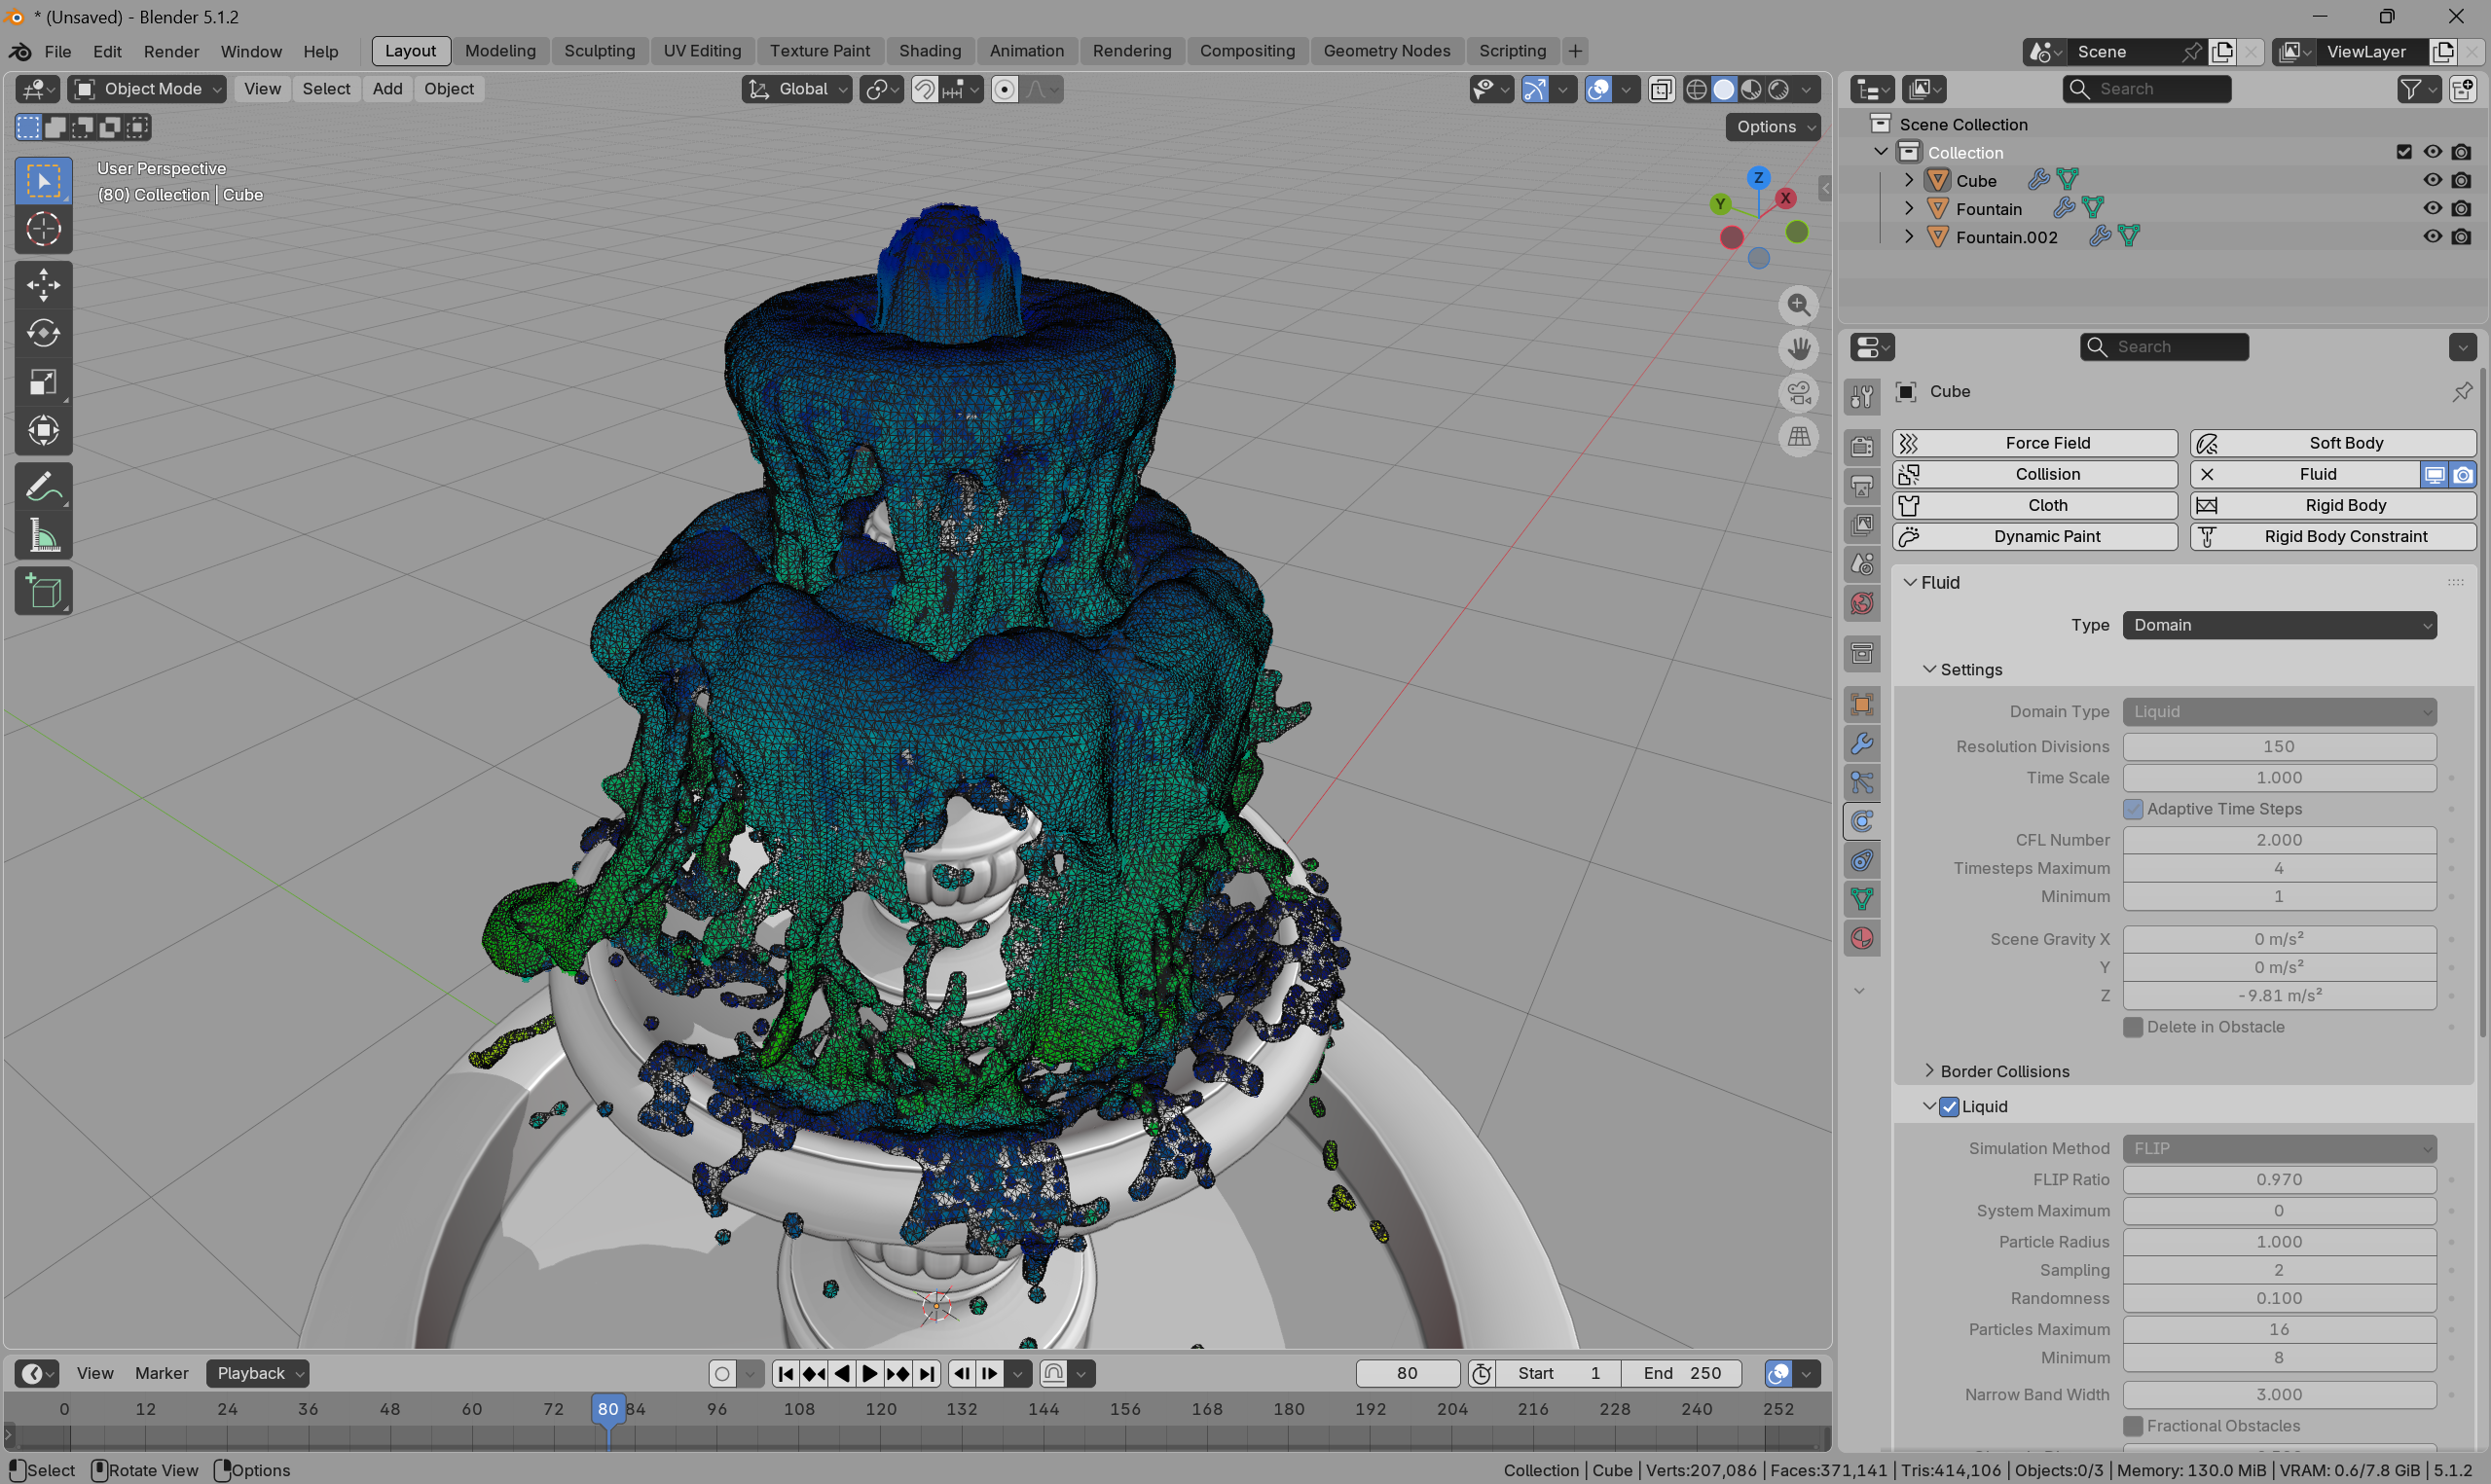
\includegraphics[width=0.85\textwidth]{figures/blender_flip.png}
    \caption{Interfejs symulacji FLIP w programie Blender z widocznym panelem konfiguracji domeny i podglądem cieczy \newline Źródło: Własne opracowanie na podstawie dokumentacji \cite{blenderdocs2023}}
    \label{fig:blender_flip}
\end{figure}

\subsection{Symulacja FLIP w silniku Unreal Engine 5}

Unreal Engine 5 jest zaawansowanym silnikiem aplikacji interaktywnych, rozwijanym przez Epic Games i 
stosowanym zarówno w produkcji gier, jak i przy tworzeniu efektów wizualnych dla filmów i symulacji \cite{ue5fluids}. 
Jednym z jego kluczowych podsystemów jest Niagara --- elastyczny system efektów wizualnych i cząsteczkowych, 
wykonujący obliczenia w całości na GPU. Możliwości symulacji cieczy udostępnia wtyczka NiagaraFluids, 
implementująca metodę FLIP dla trójwymiarowych cieczy.

Środowisko pracy oparte jest na edytorze węzłów, widocznym na rysunku~\ref{fig:ue5_flip}, 
który oferuje gotowe szablony symulacji przeznaczone do bezpośredniego umieszczenia na poziomie gry. 
Szablony te stanowią punkt wyjścia do dalszej personalizacji --- modularna architektura komponentów pozwala twórcy dostosować 
każdy aspekt symulacji do konkretnego zadania, od konfiguracji sił i warunków brzegowych, aż po modyfikację 
poszczególnych kroków solvera. Silnik jest zatem rozwiązaniem skalowalnym: 
umożliwia zarówno szybkie składanie efektów przez artystów --- osoby bez specjalistycznego
przygotowania programistycznego, konfigurujące symulację wyłącznie przez interfejs graficzny ---
jak i głębszą ingerencję algorytmiczną przez programistów efektów, którzy mają możliwość pisania
własnych modułów obliczeniowych i modyfikowania wewnętrznej logiki solvera.

\begin{figure}[ht]
    \centering
    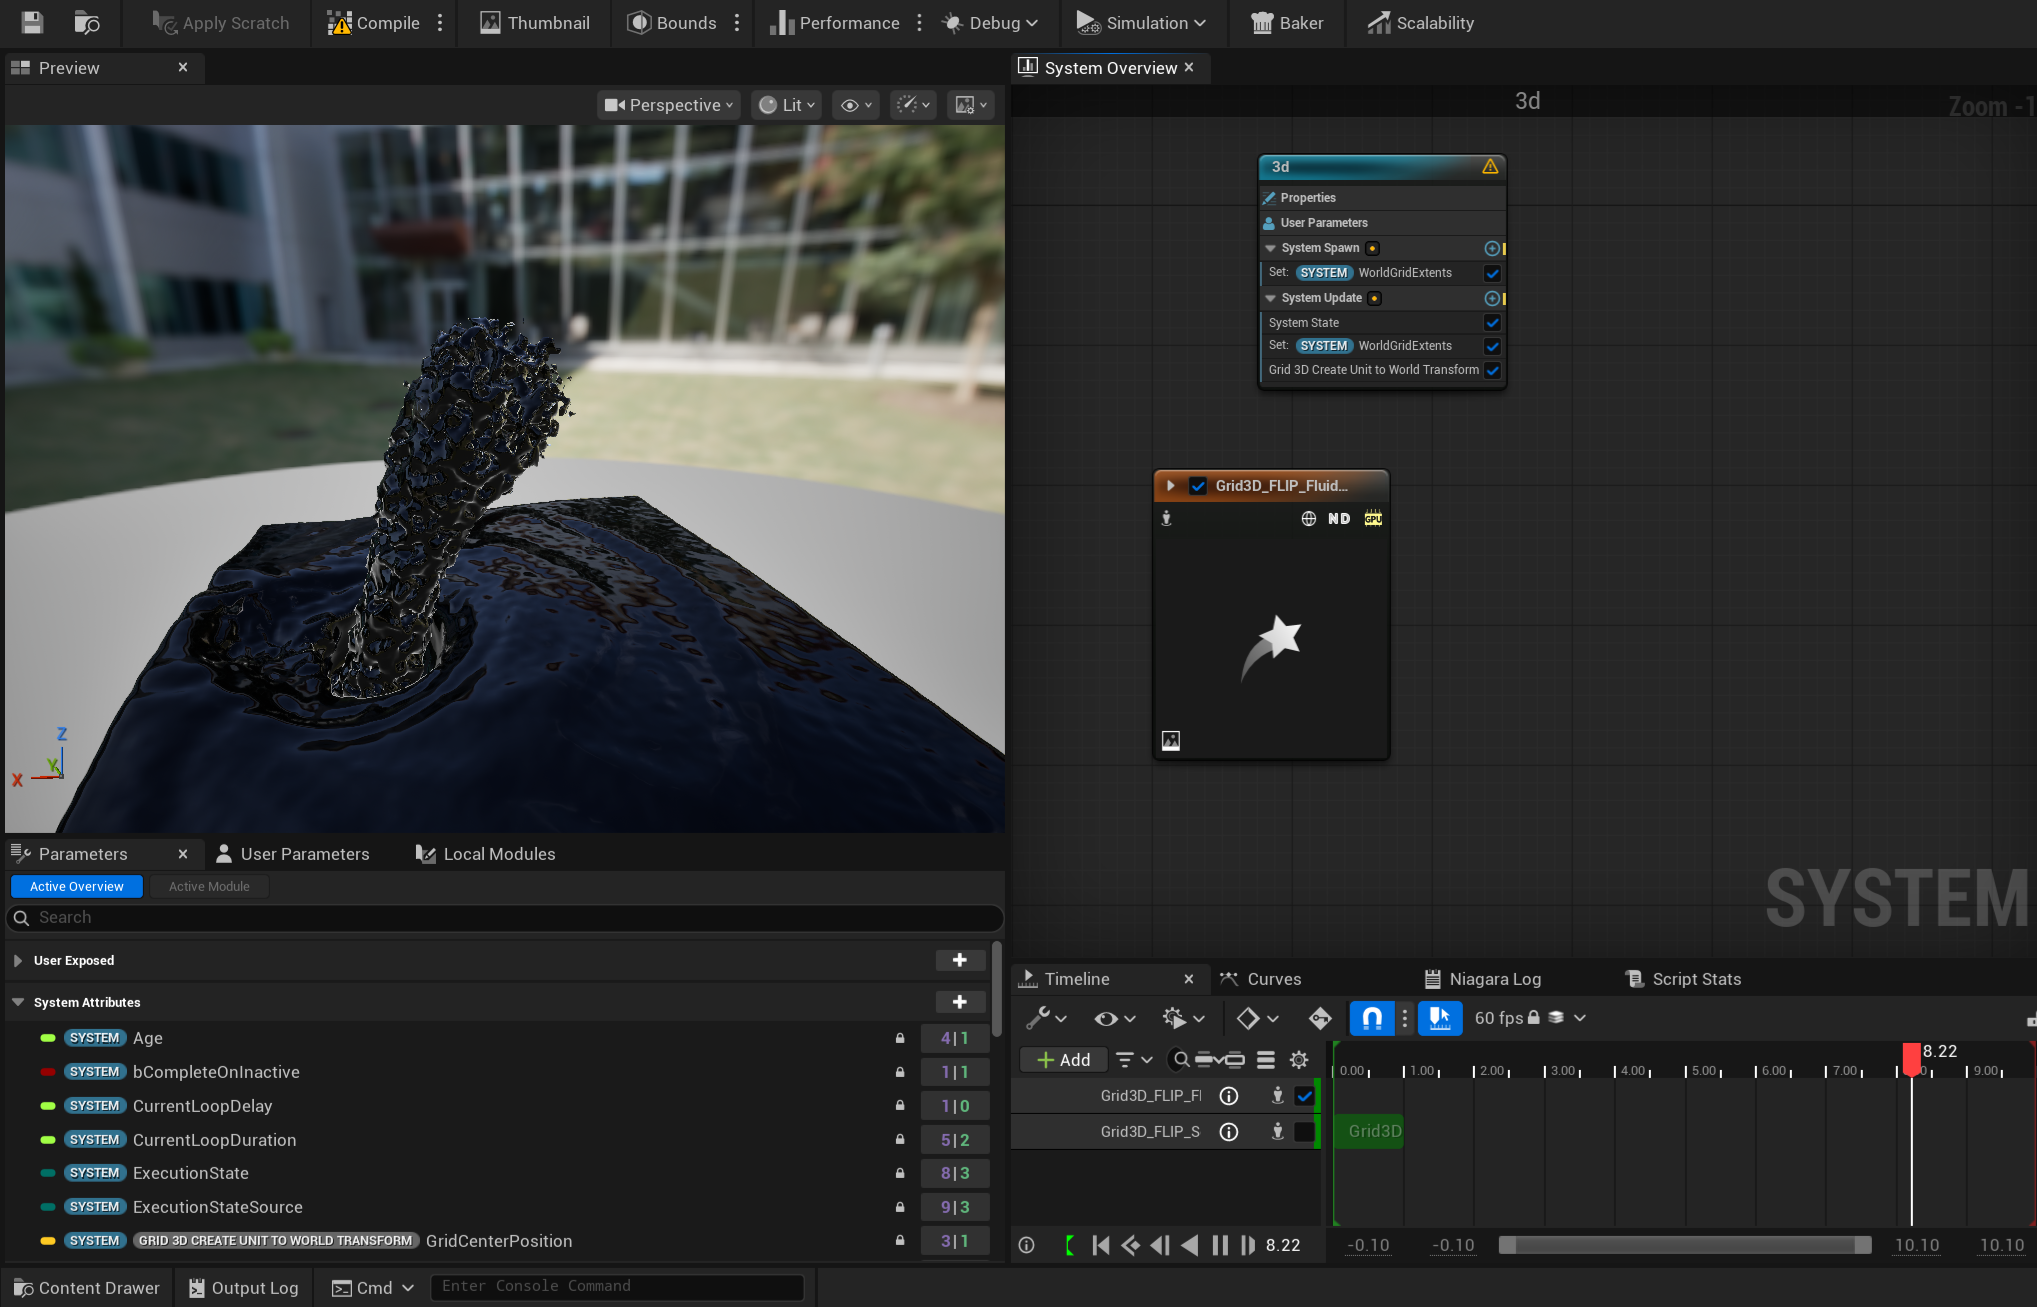
\includegraphics[width=0.85\textwidth]{figures/ue5_flip.png}
    \caption{Interfejs edytora Niagara w silniku Unreal Engine 5 z aktywną symulacją 3D FLIP zrealizowaną przy użyciu wtyczki NiagaraFluids \newline Źródło: Własne opracowanie na podstawie dokumentacji \cite{ue5fluids}}
    \label{fig:ue5_flip}
\end{figure}

\subsection{Biblioteka SPlisHSPlasH}

SPlisHSPlasH (ang.~\textit{Smoothed Particle Hydrodynamics Simulation Library}) jest 
otwartą biblioteką symulacyjną tworzoną przez grupę badawczą Jana Bendera \cite{SPlisHSPlasH_Library}. 
W odróżnieniu od dwóch poprzednich rozwiązań, biblioteka ta opiera się wyłącznie na metodzie SPH w 
formie cząsteczkowej, bez stosowania pomocniczej siatki eulerowskiej. Pod względem przyjętego modelu 
fizycznego stanowi ona najbliższy odpowiednik systemu opisanego w niniejszej pracy.

Biblioteka implementuje zestaw nowoczesnych solverów nieściśliwości, w tym m.in. DFSPH. 
Ponadto wspierane są modele fenomenologiczne lepkości, napięcia powierzchniowego i sił wirowania. 
Jej architektura opiera się wyłącznie na języku C++, a cały potok symulacyjny wykonywany jest na procesorze głównym. 
Jedynym krokiem dopuszczającym opcjonalne przeniesienie obliczeń na GPU jest wyszukiwanie sąsiedztwa, 
realizowane przez zewnętrzną bibliotekę Compact\-N\-Search --- jej wariant cu\-N\-Search umożliwia wykonanie tego 
kroku na karcie graficznej \cite{CompactNSearch_Library}. Warstwa wizualizacyjna 
korzysta z OpenGL~3.3 wyłącznie do renderowania wyników symulacji, co widoczne jest na rysunku~\ref{fig:splishsplash}. 
SPlisHSPlasH jest szeroko stosowana w środowisku naukowym jako platforma referencyjna do testowania i 
porównywania nowych algorytmów SPH \cite{koschier2020smoothed}.

\begin{figure}[ht]
    \centering
    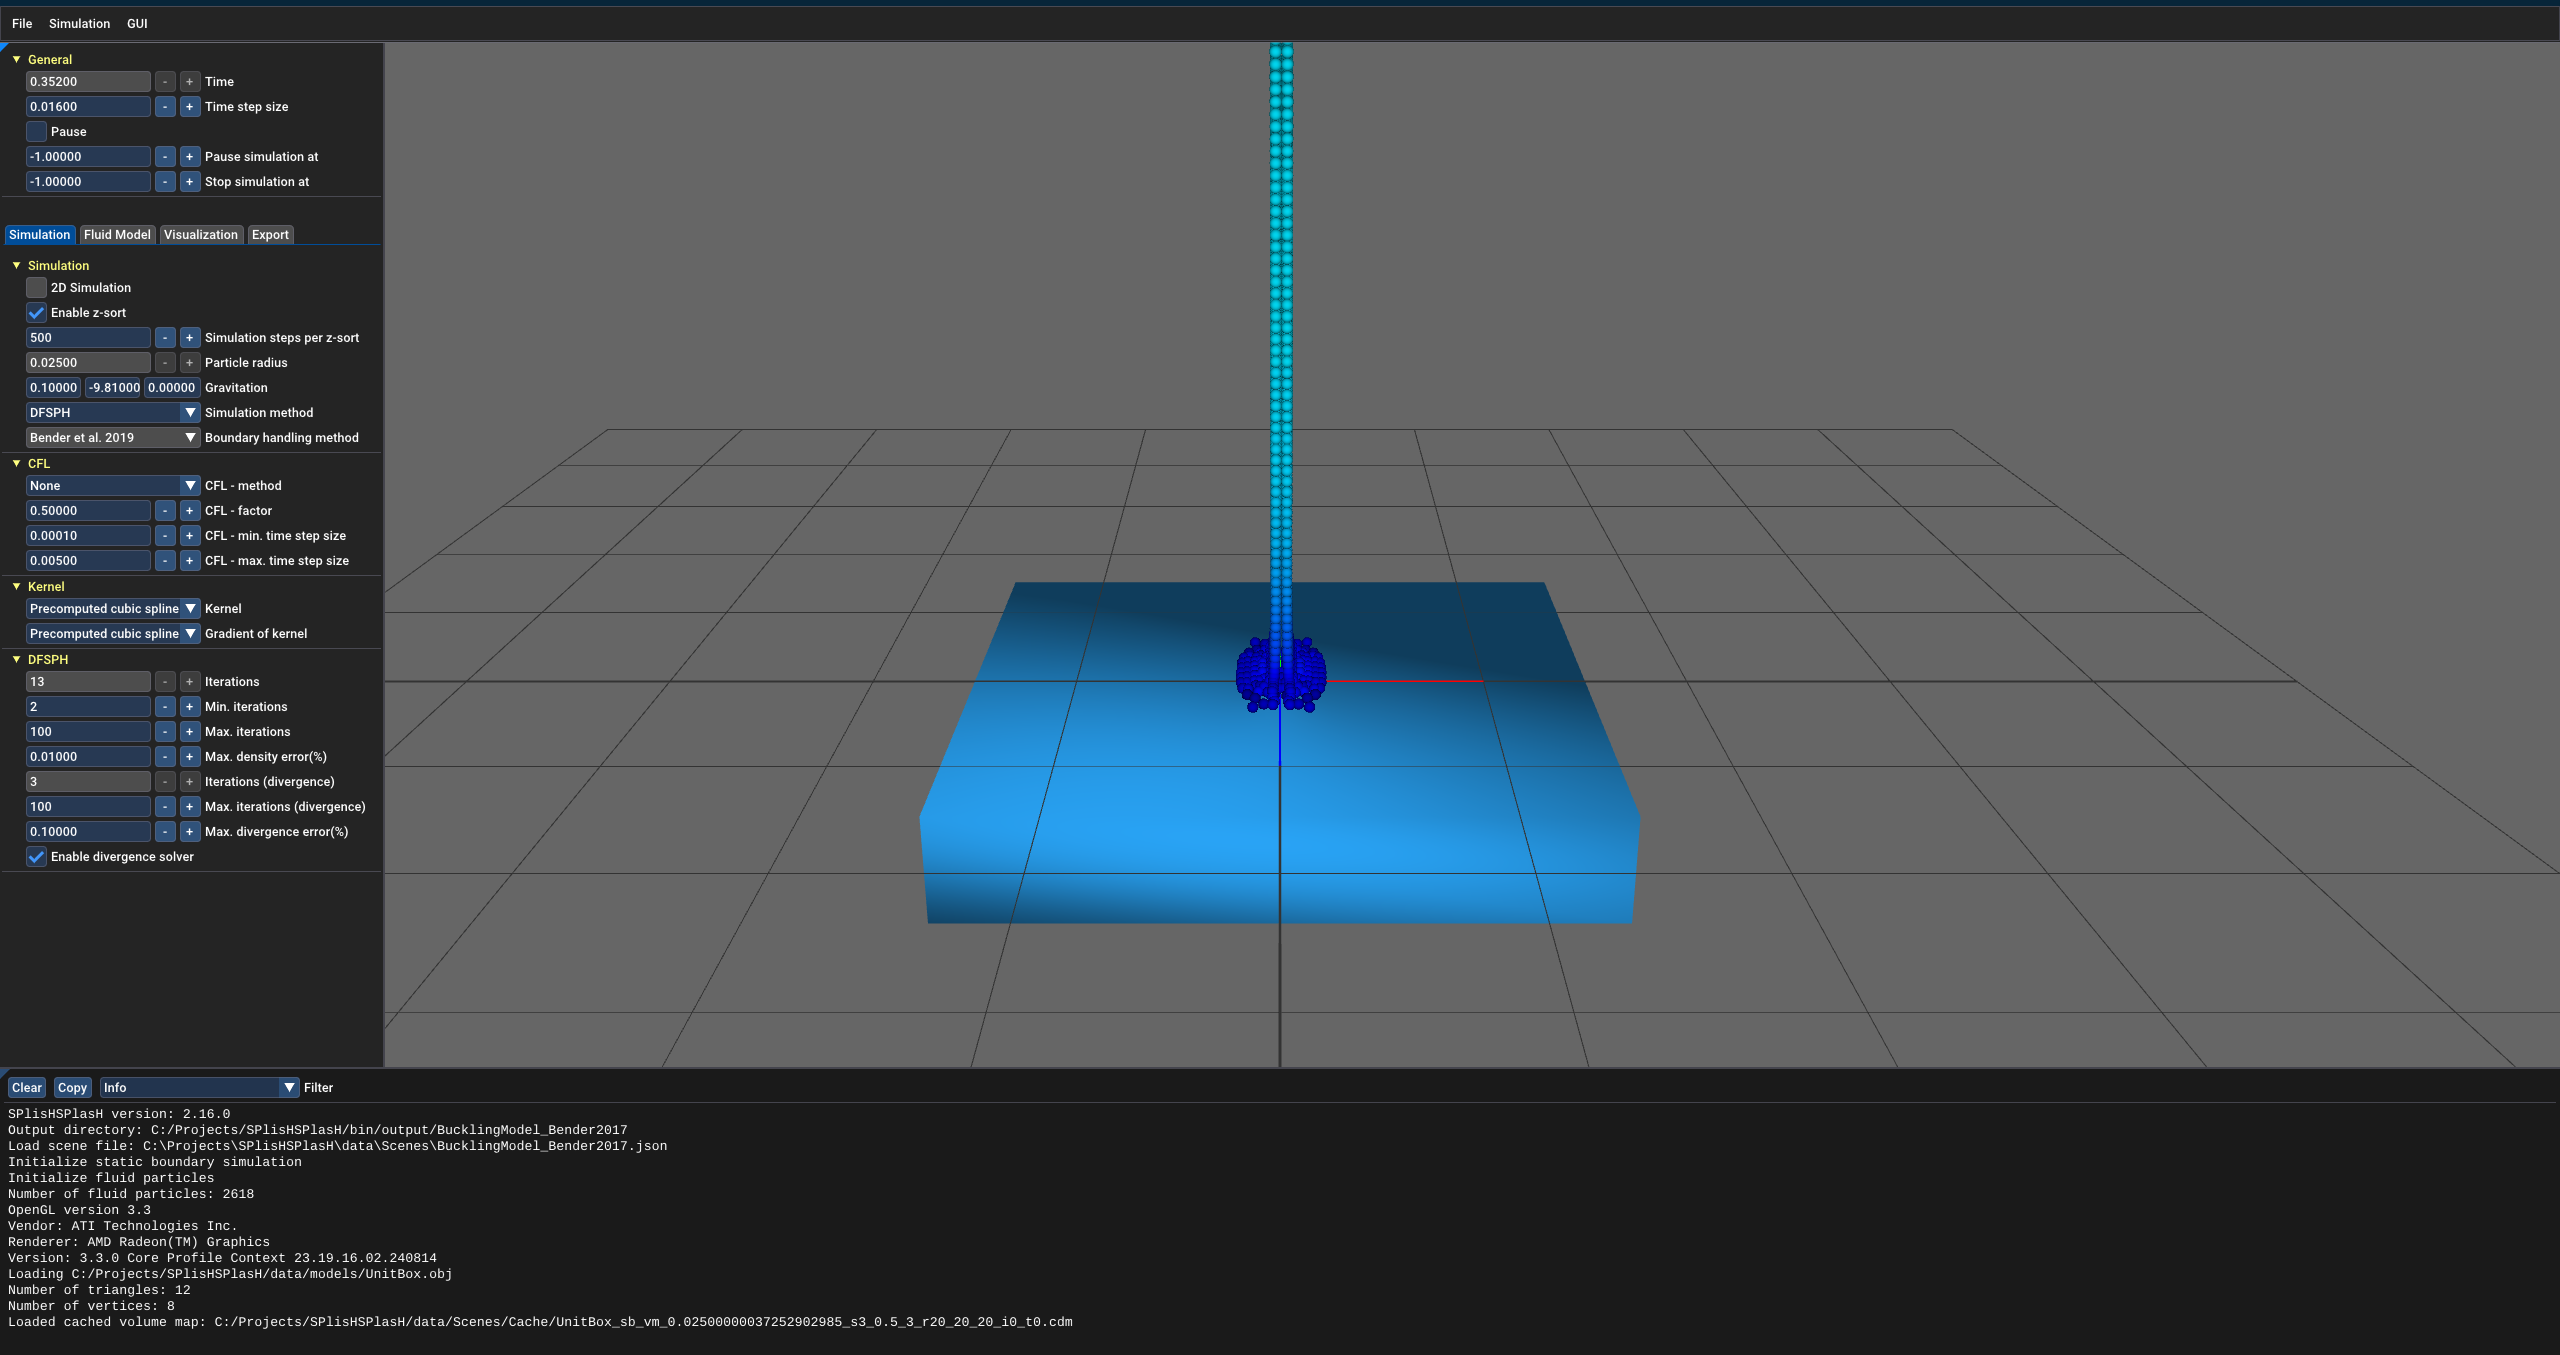
\includegraphics[width=0.85\textwidth]{figures/splishsplash.png}
    \caption{Symulacja cieczy w bibliotece SPlisHSPlasH z aktywnym solverem DFSPH i panelem konfiguracji parametrów fizycznych \newline Źródło: Własne opracowanie na podstawie dokumentacji biblioteki \cite{SPlisHSPlasH_Library}}

    \label{fig:splishsplash}
\end{figure}

\subsection{Podsumowanie rozwiązań i kontekst projektu}

Podsumowując przegląd istniejących rozwiązań, można wskazać na istotne różnice w ich architekturze oraz zastosowaniach. 
Blender jest środowiskiem nastawionym na generowanie wysokiej jakości animacji, które wymagają wcześniejszego przeliczenia.
Unreal Engine 5 z systemem Niagara oferuje wysoką wydajność w środowisku interaktywnym, lecz opiera 
się na złożonej, wysokopoziomowej architekturze silnika gry. SPlisHSPlasH z kolei jest biblioteką koncentrującą 
się na obliczeniach równoległych na procesorze w celach naukowych.

Niniejsza praca stanowi implementację algorytmu DFSPH z wykorzystaniem nowoczesnego stosu technologicznego: 
języka Rust oraz API Vulkan. W odróżnieniu od omawianych systemów, projekt skupia się na pełnym przeniesieniu 
potoku obliczeniowego na procesor graficzny przy zachowaniu niskopoziomowej kontroli nad zasobami sprzętowymi. 
Bezpośrednie porównanie cech technicznych opisanych rozwiązań z systemem opracowanym w ramach pracy przedstawiono 
w tabeli~\ref{tab:solutions_comparison}. Wybór tego podejścia wynika z chęci zbadania granic wydajności i jakości, 
jakie można osiągnąć dzięki nowoczesnym technologiom programistycznym, oraz z potrzeby stworzenia elastycznej 
platformy do dalszych eksperymentów z algorytmami SPH.

\begin{table}[ht]
    \centering
    \caption{Porównanie istniejących rozwiązań symulacji cieczy z niniejszą pracą}
    \label{tab:solutions_comparison}
    \small
    \begin{tabular}{lcccc}
    \toprule
    Cecha & Blender & Unreal Engine 5 & SPlisHSPlasH & Niniejsza praca \\ \midrule
    Metoda symulacji       & FLIP      & FLIP          & SPH       & SPH (DFSPH) \\
    Czas rzeczywisty       & Nie       & Tak           & Nie       & Tak         \\
    Obliczenia GPU         & Częściowe & Tak           & Częściowe & Tak (w pełni) \\
    Otwarte źródło         & Tak       & Tak           & Tak       & Tak         \\
    Język implementacji    & C++       & C++           & C++       & Rust        \\
    API graficzne          & OpenGL    & DX12 / Vulkan & OpenGL    & Vulkan      \\
    \bottomrule
    \end{tabular}
\end{table}

% ----------------------------------------------------------------

\section{Język programowania Rust}

Rust jest wieloparadygmatowym językiem programowania systemowego, zaprojektowanym przez pracowników Mozilla Research i opublikowanym w pierwszej stabilnej wersji w 2015 roku \cite{rust-book}. Od 2021 roku jego rozwój nadzoruje niezależna fundacja Rust Foundation. Język został stworzony z myślą o wypełnieniu niszy zajmowanej dotychczas przez C i C++ --- oferuje porównywalną wydajność obliczeniową przy jednoczesnym wyeliminowaniu całej klasy błędów wynikających z ręcznego zarządzania pamięcią.

Centralną innowacją języka jest system własności, który pozwala kompilatorowi weryfikować poprawność zarządzania pamięcią statycznie --- bez konieczności stosowania odśmiecacza pamięci. W odróżnieniu od języków zarządzanych, takich jak Java czy C\#, programy w Rust nie ponoszą kosztów przerw wywołanych odśmiecaniem. Jednocześnie, w odróżnieniu od C i C++, kompilator gwarantuje brak niezdefiniowanych zachowań w bezpiecznym kodzie: wiszące wskaźniki, przepełnienia buforów i wyścigi danych są weryfikowane statycznie i odrzucane już na etapie kompilacji. Brak wskaźników null jest egzekwowany przez typ \texttt{Option<T>}, natomiast obsługa błędów opiera się na typie \texttt{Result<T,\,E>}, wymuszającym jawne rozpatrzenie każdego przypadku wyjątkowego. Rust nie zapewnia jednak automatycznej ochrony w blokach oznaczonych jako \texttt{unsafe} --- programista przejmuje wówczas pełną odpowiedzialność za poprawność operacji niskopoziomowych, co jest niezbędne przy bezpośredniej komunikacji z API graficznym.

W odróżnieniu od języków obiektowych Rust nie posiada klas --- dane
i zachowanie są rozdzielone: struktury (ang.~\textit{structs}) przechowują
pola, a bloki \textit{impl} definiują operujące na nich metody.
Rolę interfejsów pełnią cechy (ang.~\textit{traits}) --- określają
kontrakt metod, który dowolny typ może spełnić niezależnie od swojej
wewnętrznej reprezentacji.

Ekosystem języka Rust opiera się na wbudowanym menedżerze pakietów 
Cargo oraz publicznym repozytorium crates.io. Podstawową jednostką dystrybucji
kodu jest skrzynka (ang.~\textit{crate}) --- pakiet kodu Rust przyjmujący 
formę biblioteki lub programu wykonywalnego. Repozytorium crates.io pełni rolę analogiczną 
do PyPI w Pythonie czy npm w JavaScript, pozwalając na deklaratywne zarządzanie zależnościami 
bezpośrednio w pliku konfiguracyjnym projektu, bez potrzeby instalowania zewnętrznych narzędzi. 
W niniejszym projekcie zastosowano szereg bibliotek uzupełniających. Zarządzanie oknem aplikacji 
i obsługę pętli zdarzeń zapewnia \texttt{winit} \cite{winit}. Obliczenia algebraiczne po stronie CPU, 
wektory i macierze przekształceń, realizuje \texttt{glam} \cite{glam}, biblioteka zoptymalizowana pod kątem 
instrukcji SIMD. Interfejs użytkownika do konfiguracji parametrów symulacji w czasie rzeczywistym 
zbudowano przy użyciu \texttt{egui} \cite{egui} z integracją \texttt{egui\_winit\_vulkano} \cite{egui-winit-vulkano}. 
Obsługę błędów na poziomie modułów i aplikacji upraszczają odpowiednio \texttt{thiserror} \cite{thiserror} i \texttt{anyhow} \cite{anyhow}, 
natomiast ujednoliconą infrastrukturę logowania dostarcza para \texttt{log} \cite{log-rs} i \texttt{simple\_logger} \cite{simple-logger}.

\begin{table}[ht]
    \centering
    \caption{Porównanie języków Rust i C++ pod względem cech istotnych dla programowania systemowego}
    \label{tab:rust_vs_cpp}
    \small
    \begin{tabular}{lcc}
    \toprule
    Cecha & C++ & Rust \\ \midrule
    Bezpieczeństwo pamięci      & Manualne              & Gwarantowane przez kompilator \\
    Odśmiecacz pamięci          & Nie                   & Nie                           \\
    Niezdefiniowane zachowania  & Możliwe               & Niemożliwe (safe Rust)        \\
    Wyścigi danych              & Możliwe               & Niemożliwe (czas kompilacji)  \\
    Wskaźniki null              & Tak                   & Nie (\texttt{Option<T>})      \\
    Zerowe koszty abstrakcji    & Tak                   & Tak                           \\
    Standardowy menedżer pakietów & Brak                & Cargo                         \\
    Dojrzałość ekosystemu       & Wysoka (od 1983)      & Rosnąca (od 2015)             \\
    \bottomrule
    \end{tabular}
\end{table}

Rust jest coraz powszechniej postrzegany jako naturalny następca C++ w nowych projektach systemowych. Organizacje takie jak Microsoft, Google i Linux Foundation włączyły go już do swoich stosów technologicznych jako odpowiedź na rosnące wymagania w zakresie bezpieczeństwa oprogramowania. Jako język oferujący zerowe koszty abstrakcji, rozbudowany system typów i statyczne gwarancje poprawności bez narzutu czasowego, Rust eliminuje całą klasę błędów trudnych do debugowania w złożonych systemach wielowątkowych - co czyni go szczególnie trafnym wyborem dla implementacji silnika symulacji cieczy opisanego w niniejszej pracy.

% ----------------------------------------------------------------

\section{API graficzne Vulkan}

Vulkan jest niskopoziomowym, wieloplatformowym interfejsem programowania graficznego, 
opracowanym przez konsorcjum Khronos Group i opublikowanym w 2016 roku \cite{vulkan-spec}. 
Jego geneza wynika z narastających ograniczeń architektury OpenGL, 
która przez ponad dwie dekady rozrastało się o kolejne warstwy abstrakcji i 
niejawne mechanizmy zarządzania zasobami. Sterownik OpenGL pełnił rolę rozbudowanego 
pośrednika: sam synchronizował polecenia GPU, podejmował decyzje o alokacji pamięci i 
kompilował shadery w nieokreślonych momentach, co prowadziło do znacznego narzutu procesora głównego, 
uniemożliwiało efektywną wielowątkowość i skutkowało nieprzewidywalnym zachowaniem w sytuacjach granicznych. 
Bezpośrednim poprzednikiem Vulkana jest biblioteka Mantle \cite{amdmantle2015}, opracowana przez AMD we współpracy z~deweloperami 
gier w 2013 roku, stanowiąca pierwszą propozycję niskopoziomowego API graficznego, która wykazała, 
że jawne przejęcie przez programistę kontroli nad sprzętem przekłada się na mierzalne zyski wydajnościowe.

Centralną filozofią Vulkana jest jawność i determinizm. Każdy zasób, taki jak bufor pamięci, 
obraz, potok obliczeniowy, jest tworzony i zarządzany przez programistę w sposób jawny, 
a każda operacja synchronizacji między procesorem a GPU musi być ręcznie zdefiniowana. 
Rezygnacja z globalnego automatu stanów na rzecz izolowanych, niezależnych obiektów umożliwia 
równoległe budowanie potoków poleceń w wielu wątkach bez ryzyka konfliktu stanu. 
Ujednoliconym wzorcem inicjalizacji w API Vulkan jest wykorzystanie struktur opisowych. 
Tworzenie dowolnego obiektu wymaga od programisty wypełnienia~dedykowanej struktury konfiguracyjnej, 
która precyzyjnie definiuje jego parametry, a następnie przekazania jej do odpowiedniej funkcji tworzącej. 
Podejście to, stosowane konsekwentnie w całym standardzie, sprawia, że konfiguracja systemu jest w pełni jawna. 
Pozwala to na precyzyjne określenie zależności między obiektami już na poziomie kodu, co eliminuje domyślne stany 
sterownika graficznego.

Drugą fundamentalną cechą Vulkana jest system rozszerzeń, zaprojektowany jako integralna 
część architektury API od pierwszej wersji specyfikacji. Rdzeń Vulkana jest celowo minimalny i stabilny: 
obejmuje wyłącznie operacje wspólne dla wszystkich implementacji sprzętowych. 
Wszelkie funkcjonalności specyficzne dla producenta lub nowsze możliwości renderowania 
udostępniane są przez rozszerzenia aktywowane jawnie przy tworzeniu instancji lub urządzenia. 
Rozszerzenia dzielą się na trzy kategorie: rozszerzenia producenta sprzętu (np.\ \texttt{VK\_NV\_*} lub
\texttt{VK\_AMD\_*}), rozszerzenia wieloproducentowe (\texttt{VK\_EXT\_*}) oraz rozszerzenia
ratyfikowane przez Khronos (\texttt{VK\_KHR\_*}).

Ostatnia kategoria powstaje w~drodze konsensusu wszystkich członków organizacji Khronos~---
AMD, NVIDIA, Intel, ARM, Google, Apple i~innych --- i~pełni dwojaką rolę.
Po pierwsze, dostarcza krytyczne funkcjonalności obsługiwane przez wszystkie współczesne karty graficzne,
które z~różnych powodów nie trafiły do rdzenia specyfikacji; przykładem jest \texttt{VK\_KHR\_swapchain}
umożliwiający prezentację obrazu na ekranie systemu operacyjnego, czy \texttt{VK\_KHR\_ray\_tracing\_pipeline}
wprowadzający sprzętowe śledzenie promieni.
Po drugie, rozszerzenia \texttt{KHR} pełnią rolę oficjalnej ,,\textit{poczekalni}'' dla nowych technologii:
zamiast pospiesznie modyfikować stabilny rdzeń, Khronos publikuje rozszerzenie, pozwala deweloperom
je przetestować w~warunkach produkcyjnych, a~jeśli okaże się ono dojrzałe~--- włącza je do kolejnej
wersji specyfikacji rdzeniowej (ang.~\textit{core specification}). Mechanizm ten był stosowany konsekwentnie 
w~wersjach Vulkan 1.1, 1.2 i~1.3, do których przeniesiono łącznie kilkadziesiąt wcześniejszych rozszerzeń \texttt{KHR}.

Podejście to umożliwia producentom sprzętu udostępnianie możliwości swoich układów
bez naruszania globalnej kompatybilności, pozwalając jednocześnie programiście na jawne deklarowanie
funkcjonalności wymaganych przez aplikację.

\subsection{Instancja, urządzenie fizyczne i logiczne}
\label{sec:vulkan_hierarchy}

\texttt{VkInstance} jest punktem wejścia do środowiska uruchomieniowego Vulkana i
korzeniem całej hierarchii obiektów API. Jej utworzenie ładuje sterownik Vulkana
i inicjalizuje rozszerzenia działające na poziomie instancji, które dotyczą
platformy systemowej, a nie konkretnego układu graficznego. Przykładem jest
\texttt{VK\_KHR\_surface}, które definiuje abstrakcję powierzchni okienkowej niezależną
od systemu operacyjnego, oraz towarzyszące mu rozszerzenia platformowe, takie jak
\texttt{VK\_KHR\_win32\_surface} czy \texttt{VK\_KHR\_xcb\_surface}, odpowiadające
za integrację z konkretnym podsystemem okienkowym. Rozszerzenia instancji
aktywuje się przy jej tworzeniu, deklarując ich nazwy w strukturze \texttt{VkInstanceCreateInfo}.

Po utworzeniu instancji możliwe jest wyliczenie dostępnych urządzeń fizycznych.
\texttt{VkPhysicalDevice} reprezentuje jeden fizyczny układ graficzny widoczny dla systemu.
Na stacji roboczej może znajdować się kilka takich układów, w tym zintegrowany procesor 
graficzny wbudowany w jednostkę centralną oraz dedykowana karta graficzna. Vulkan pozwala
programiście odpytać każde z nich o właściwości: typ urządzenia (dyskretna karta graficzna,
układ zintegrowany, CPU), limity sprzętowe, obsługiwane formaty obrazów i funkcjonalności.
Na tej podstawie aplikacja może samodzielnie wybrać najbardziej odpowiedni układ lub
umożliwić taki wybór użytkownikowi.

Wykorzystując wybrany układ fizyczny, programista tworzy urządzenie logiczne
\texttt{VkDevice}, stanowiące centralny obiekt API, z którym powiązane są wszystkie kolejki poleceń, 
bufory, obrazy oraz potoki obliczeniowe. Na tym etapie aktywowane są
rozszerzenia działające na poziomie urządzenia, czyli dotyczące możliwości konkretnego
układu graficznego. Rozróżnienie poziomów ma praktyczne znaczenie: \texttt{VK\_KHR\_surface}
jest rozszerzeniem instancji, bo integracja z oknem systemu operacyjnego jest kwestią
platformową; \texttt{VK\_KHR\_swapchain}, czyli mechanizm prezentowania klatek na ekranie,
jest już rozszerzeniem urządzenia, bo wymaga fizycznego wyjścia wyświetlacza. Układ
graficzny w serwerze bez monitora może nie obsługiwać \texttt{VK\_KHR\_swapchain} w ogóle,
lecz nadal będzie w pełni zdolny do obliczeń ogólnego przeznaczenia na GPU. Taki podział
pozwala aplikacji jawnie deklarować wymagane zależności sprzętowe zamiast zakładać
obecność możliwości, których dany układ może nie posiadać.
Relację między trzema warstwami inicjalizacyjnymi ilustruje rysunek~\ref{fig:vulkan_hierarchy}.

\begin{figure}[ht]
\centering
\begin{tikzpicture}[
  vkbox/.style={rectangle, draw=black!80, fill=white, rounded corners=3pt,
    minimum width=4.4cm, minimum height=0.72cm, align=center, font=\small\ttfamily},
  vkfade/.style={rectangle, draw=black!25, fill=gray!6, text=black!30, rounded corners=3pt,
    minimum width=4.4cm, minimum height=0.72cm, align=center, font=\small\ttfamily},
  resbox/.style={rectangle, draw=black!80, fill=white, rounded corners=3pt,
    minimum width=3.2cm, minimum height=0.72cm, align=center, font=\small\ttfamily},
  arr/.style={->, >=Stealth, semithick},
  faint/.style={->, >=Stealth, semithick, draw=black!25}
]
  \node[vkbox]  (inst)  at (0,      0)   {VkInstance};
  \node[vkbox]  (phys0) at (-3.2,  -2.0) {VkPhysicalDevice [0]};
  \node[vkfade] (phys1) at ( 3.2,  -2.0) {VkPhysicalDevice [1]};
  \node[vkbox]  (dev)   at (0,     -4.0) {VkDevice};
  \node[resbox] (queue) at (-3.6,  -5.9) {VkQueue};
  \node[resbox] (res)   at (0,     -5.9) {VkBuffer,~VkImage};
  \node[resbox] (pipe)  at ( 3.6,  -5.9) {VkPipeline};

  \draw[arr]   (inst)  -- (phys0);
  \draw[faint] (inst)  -- (phys1);
  \draw[arr]   (phys0) -- (dev);
  \draw[arr]   (dev)   -- (queue);
  \draw[arr]   (dev)   -- (res);
  \draw[arr]   (dev)   -- (pipe);
\end{tikzpicture}
\caption{Hierarchia inicjalizacyjna Vulkana. Instancja daje dostęp do urządzeń fizycznych,
z których jedno wybierane jest do utworzenia urządzenia logicznego \texttt{VkDevice}, będącego
punktem zaczepu wszystkich pozostałych obiektów API. Szary węzeł oznacza niewybrany układ fizyczny
\newline Źródło: Opracowanie własne na podstawie specyfikacji \cite{vulkan-spec}}
\label{fig:vulkan_hierarchy}
\end{figure}

\subsection{Kolejki i pule poleceń}

Nowoczesne karty graficzne udostępniają wiele sprzętowych kolejek poleceń, przez które
procesor przekazuje pracę do wykonania na GPU. Vulkan grupuje je w rodziny kolejek, 
z których każda obsługuje określony zestaw operacji. Typowa karta graficzna eksponuje co 
najmniej rodzinę graficzną, obsługującą rysowanie i prezentację klatek, oraz rodzinę obliczeniową, 
przeznaczoną do obliczeń ogólnego przeznaczenia. Wiele układów udostępnia też 
wyspecjalizowaną rodzinę transferową, zoptymalizowaną sprzętowo do kopiowania danych
między pamięcią systemową procesora głównego a~dedykowaną pamięcią karty graficznej.
W nomenklaturze Vulkana strona procesorowa systemu, obejmująca procesor główny i pamięć RAM,
określana jest terminem \textit{host}, zaś strona układu graficznego wraz z jego pamięcią
wideo terminem \textit{device}.
Programista odpytuje wybrany \texttt{VkPhysicalDevice} o dostępne rodziny i deklaruje,
z których z nich chce korzystać, w strukturze \texttt{VkDeviceCreateInfo} przekazywanej
przy tworzeniu urządzenia logicznego. Efektem jest zbiór uchwytów \texttt{VkQueue},
z których każdy reprezentuje jedną kolejkę danej rodziny.

Samo polecenie nie jest przekazywane do kolejki bezpośrednio jako wywołanie funkcji.
Zamiast tego Vulkan stosuje model rejestrowania odroczonych poleceń. Programista tworzy
\texttt{VkCommandPool}, obiekt zarządzający pamięcią przeznaczoną na polecenia, powiązany
z konkretną rodziną kolejek. Z puli tej alokowane są bufory poleceń \texttt{VkCommandBuffer},
w których rejestruje się sekwencje operacji GPU. Operacje te obejmują przesłania danych
między buforami, bariery synchronizacji, uruchomienia potoków graficznych oraz wywołania
obliczeniowe, określane terminem \textit{dispatch}. Bufor poleceń rejestruje całą sekwencję
operacji po stronie procesora głównego, a następnie przekazywany jest do kolejki jednym
wywołaniem funkcji wysyłającej. GPU przetwarza zarejestrowane polecenia asynchronicznie
względem procesora, co jest zasadniczą różnicą w stosunku do modelu OpenGL, gdzie każde
wywołanie API było natychmiastowym żądaniem wykonywanym przez sterownik.

Rozdzielenie rejestrowania od wysyłania przynosi dwie praktyczne konsekwencje. Po pierwsze,
wiele wątków procesora może jednocześnie rejestrować polecenia w niezależnych buforach,
korzystając z osobnych pul powiązanych z tą samą rodziną kolejek. Po drugie, bufor poleceń
reprezentujący stały zestaw pracy, który nie zmienia się między klatkami, może być
zarejestrowany raz i wysyłany wielokrotnie bez ponownego budowania.

\subsection{Łańcuch wymiany i dynamiczne renderowanie}
\label{sec:vulkan_swapchain}

Renderowanie w czasie rzeczywistym polega na cyklicznym generowaniu kolejnych obrazów klatki
i przesyłaniu ich na ekran. Konieczność synchronizacji tego procesu z monitorem wynika
z fundamentalnej właściwości sprzętu wyświetlającego: monitor odświeża obraz ze stałą
częstotliwością, odczytując zawartość bufora wideo z pamięci karty graficznej.
Jeśli aplikacja zapisuje nową klatkę bezpośrednio do obszaru, który monitor właśnie odczytuje,
na ekranie pojawia się artefakt rozrywania obrazu (ang.~\textit{screen tearing}):
górna część klatki pochodzi z poprzedniego obrazu, a dolna z~aktualnie zapisywanego.
Rozwiązaniem jest oddzielenie bufora wyświetlanego od bufora roboczego i podmiana ich zawartości
dopiero po zakończeniu cyklu odświeżania. W odróżnieniu od OpenGL, które ukrywało ten
mechanizm za pojęciem domyślnego bufora ramki, Vulkan wymaga jawnego skonstruowania tej
infrastruktury w postaci łańcucha wymiany (ang.~\textit{swapchain}).

Łańcuch wymiany jest zestawem obrazów zarządzanych przez system okienkowy, przeznaczonych
do prezentacji na ekranie. Aplikacja pobiera jeden z dostępnych obrazów, rysuje do niego
klatkę, a następnie oddaje go do kolejki prezentacji, skąd trafia on na ekran w odpowiednim
momencie. Liczba obrazów w łańcuchu jest konfigurowalna: przy dwóch obrazach jeden jest
wyświetlany, a drugi przygotowywany, co określa się mianem podwójnego buforowania
(ang.~\textit{double buffering}); przy trzech obrazach aplikacja może przygotowywać kolejną klatkę
jeszcze zanim poprzednio złożona dotrze na ekran, co nosi nazwę potrójnego buforowania
(ang.~\textit{triple buffering}) i zmniejsza ryzyko przestojów renderowania kosztem nieznacznie
wyższego opóźnienia. Sposób synchronizacji z częstotliwością odświeżania monitora określa
tryb prezentacji: tryb \texttt{FIFO} odpowiada klasycznej synchronizacji pionowej, a tryb
\texttt{MAILBOX} zastępuje oczekujący obraz nowszym, jeśli ten jest już gotowy, minimalizując
widoczne opóźnienie klatki.

Vulkan oferuje dwa podejścia do przekazania poleceń rysowania do obrazu łańcucha wymiany:
model tradycyjny oparty na jawnie skompilowanych obiektach przejścia renderowania i bufora ramki
oraz dynamiczne renderowanie, wprowadzone jako funkcja rdzeniowa w wersji 1.3.
W modelu tradycyjnym przejście renderowania (\texttt{VkRenderPass}) jest deklaratywnym opisem struktury operacji
rysowania: definiuje, jakie załączniki obrazowe będą używane, w jakim formacie, co ma się
stać z ich zawartością na początku przejścia (wyczyszczenie lub zachowanie) i na końcu
(zachowanie lub odrzucenie). Opis ten jest kompilowany przez sterownik z wyprzedzeniem,
co pozwala mu na optymalizację dostępów do pamięci. Bufor ramki (\texttt{VkFramebuffer})
wiąże konkretne widoki obrazów (\texttt{VkImageView}) z załącznikami zadeklarowanymi
w przejściu renderowania. Ponieważ łańcuch wymiany dostarcza zestaw obrazów, a nie jeden,
aplikacja tworzy osobny bufor ramki dla każdego obrazu w łańcuchu i wybiera właściwy
przy budowaniu bufora poleceń danej klatki.
Oba podejścia, tradycyjne i dynamiczne, zestawia rysunek~\ref{fig:vulkan_rendering_path}.

\begin{figure}[ht]
\centering
\begin{tikzpicture}[
  fbox/.style={rectangle, draw=black!80, fill=white, rounded corners=3pt,
    minimum width=4.6cm, minimum height=0.72cm, align=center, font=\small\ttfamily},
  hbox/.style={rectangle, draw=black!80, fill=gray!14, rounded corners=3pt,
    minimum width=4.6cm, minimum height=0.72cm, align=center, font=\small\ttfamily},
  mbox/.style={rectangle, draw=black!60, fill=black!6, rounded corners=3pt,
    minimum width=4.6cm, minimum height=0.72cm, align=center, font=\small\sffamily},
  arr/.style={->, >=Stealth, semithick},
  tit/.style={font=\small\bfseries\sffamily, align=center}
]
  \node[tit] at (-3.0,  0.5) {Tradycyjny model};
  \node[tit] at ( 3.0,  0.5) {Dynamiczne renderowanie};
  \draw[black!18, dashed, thin] (0, 0.85) -- (0, -6.1);

  % --- Left column ---
  \node[fbox] (ls) at (-3.0, -0.40) {VkImage (swapchain)};
  \node[fbox] (lv) at (-3.0, -1.35) {VkImageView};
  \node[hbox] (lr) at (-3.0, -2.30) {VkRenderPass};
  \node[hbox] (lf) at (-3.0, -3.25) {VkFramebuffer};
  \node[fbox] (lc) at (-3.0, -4.20) {Komendy rysowania};
  \node[mbox] (lm) at (-3.0, -5.30) {Monitor};

  \draw[arr] (ls) -- (lv);
  \draw[arr] (lv) -- (lr);
  \draw[arr] (lr) -- (lf);
  \draw[arr] (lf) -- (lc);
  \draw[arr] (lc) -- (lm);

  % --- Right column ---
  \node[fbox] (rs) at (3.0, -0.40)  {VkImage (swapchain)};
  \node[fbox] (rv) at (3.0, -1.35)  {VkImageView};
  \node[fbox] (rd) at (3.0, -2.775) {vkCmdBeginRendering};
  \node[fbox] (rc) at (3.0, -4.20)  {Komendy rysowania};
  \node[mbox] (rm) at (3.0, -5.30)  {Monitor};

  \draw[arr] (rs) -- (rv);
  \draw[arr] (rv) -- (rd);
  \draw[arr] (rd) -- (rc);
  \draw[arr] (rc) -- (rm);
\end{tikzpicture}
\caption{Porównanie ścieżek renderowania w Vulkanie. Zacienione pola w modelu tradycyjnym
(\texttt{VkRenderPass} i \texttt{VkFramebuffer}) są zbędne w dynamicznym renderowaniu,
które deklaruje załączniki bezpośrednio w buforze poleceń
\newline Źródło: Opracowanie własne na podstawie specyfikacji \cite{vulkan-spec}}
\label{fig:vulkan_rendering_path}
\end{figure}

W modelu dynamicznego renderowania programista deklaruje używane załączniki bezpośrednio
w buforze poleceń, tuż przed poleceniami rysowania, zamiast opisywać je z wyprzedzeniem
w dedykowanym obiekcie kompilowanym przez sterownik. Eliminuje to potrzebę utrzymywania
zgodności między przejściami renderowania a potokami graficznymi i lepiej odpowiada
architekturom, w których zestaw załączników zmienia się między krokami renderowania.

\subsection{Zasoby: bufory, obrazy i deskryptory}

Pojęcie \texttt{VkImage} pojawiło się już przy omawianiu łańcucha wymiany jako kontener
klatki gotowej do prezentacji. W szerszym sensie obraz jest zasobem GPU reprezentującym
wielowymiarową tablicę danych pikselowych, opisaną formatem (np.\ \texttt{VK\_FORMAT\_R32\_SFLOAT}),
rozmiarem i liczbą poziomów mipmap (prekalkulowanych kopii obrazu w malejących rozdzielczościach). 
Sprzęt przechowuje obrazy w wewnętrznym układzie
kafelkowym, zoptymalizowanym pod kątem lokalności dostępów podczas próbkowania i zapisu.
Programista nie adresuje obrazu bezpośrednio: każdy dostęp odbywa się przez
\texttt{VkImageView}, który deklaruje format interpretacji i zakres odczytywanego podzasobu.

Bufor (\texttt{VkBuffer}) jest ciągłym obszarem pamięci GPU bez narzuconej struktury
wewnętrznej. Jego semantykę określają flagi użycia przekazane przy tworzeniu oraz sposób,
w jaki shadery go odczytują i zapisują. Tworzenie bufora składa się z dwóch etapów:
najpierw tworzy się obiekt \texttt{VkBuffer} opisujący rozmiar i zamierzone użycie,
a następnie przydziela się mu pamięć wybraną z odpowiedniego stosu. Vulkan eksponuje
wiele stosów pamięci o różnych własnościach: pamięć lokalna dla urządzenia
(ang.~\textit{device-local}) rezyduje wyłącznie po stronie układu graficznego
i oferuje najwyższą przepustowość, natomiast pamięć widoczna dla procesora
(ang.~\textit{host-visible}) jest dostępna do bezpośredniego zapisu przez procesor główny.
W praktyce zarządzanie tym procesem deleguje się do biblioteki Vulkan Memory Allocator~(VMA) \cite{vma-library},
opracowanej przez AMD: programista deklaruje wyłącznie przeznaczenie bufora,
a VMA dobiera właściwy stos pamięci i zarządza jego fragmentacją.
Aby załadować dane przygotowane po stronie procesora do bufora rezydującego w pamięci
lokalnej dla urządzenia, stosuje się bufor pośredniczący (ang.~\textit{staging buffer}):
tymczasowy bufor w pamięci widocznej dla procesora, wypełniany przez CPU, którego
zawartość kopiowana jest następnie przez rodzinę kolejek transferowych do docelowej
pamięci układu graficznego.

Flagi użycia determinują dozwolone operacje na buforze i wpływają na wybór stosu pamięci
przez VMA. Tabela~\ref{tab:buffer_types} zestawia typy buforów istotne dla niniejszej
implementacji.

\begin{table}[ht]
\centering
\caption{Typy buforów Vulkana i ich zastosowanie}
\label{tab:buffer_types}
\small
\begin{tabular}{lp{9.5cm}}
\toprule
Typ bufora & Zastosowanie \\
\midrule
Wierzchołkowy & Dane wierzchołków przekazywane bezpośrednio do potoku graficznego \\ 
\addlinespace
Jednorodny (UBO) & Małe, stałe dane odczytywane w shaderach: macierze transformacji, parametry symulacji \\
\addlinespace
Składowania (SSBO) & Duże dane dostępne do odczytu i zapisu w shaderach obliczeniowych; główny nośnik stanu symulacji \\
\addlinespace
Pośredniczący (Staging) & Tymczasowy bufor w pamięci host-visible służący do transferu danych inicjalizacyjnych z CPU do pamięci device-local \\
\bottomrule
\end{tabular}
\end{table}

Shadery nie adresują buforów i obrazów bezpośrednio przez wskaźnik; zasoby te wiązane są
z potokiem obliczeniowym za pośrednictwem zestawów deskryptorów.
Schemat powiązań deklarowany jest w obiekcie \texttt{VkDescriptorSetLayout}, który precyzuje,
jakiego rodzaju zasoby oczekiwane są na każdym miejscu wiązania shaderów.
Alokacją zestawów zarządza \texttt{VkDescriptorPool}: obiekt rezerwujący z góry blok pamięci
przeznaczony wyłącznie na zestawy danego układu, analogicznie do roli,
jaką \texttt{VkCommandPool} pełni wobec buforów poleceń.
Z puli alokowany jest \texttt{VkDescriptorSet}, wiążący konkretne uchwyty
\texttt{VkBuffer} i \texttt{VkImageView} ze zdefiniowanymi miejscami wiązania.
Układ potoków \texttt{VkPipelineLayout} agreguje jeden lub kilka takich układów zestawów
i jest wbudowywany w każdy potok obliczeniowy przy jego tworzeniu, dzięki czemu sterownik
zna pełen schemat zasobów wymaganych przez shadery już na etapie kompilacji.
Zależności między wymienionymi obiektami ilustruje rysunek~\ref{fig:vulkan_resources}.

\begin{figure}[ht]
\centering
\begin{tikzpicture}[
  vkbox/.style={rectangle, draw=black!80, fill=white, rounded corners=3pt,
    minimum width=4.0cm, minimum height=0.72cm, align=center, font=\small\ttfamily},
  mbox/.style={rectangle, draw=black!60, fill=black!7, rounded corners=3pt,
    minimum width=4.6cm, minimum height=0.72cm, align=center, font=\small\sffamily},
  arr/.style={->, >=Stealth, semithick},
  refarr/.style={->, >=Stealth, semithick, dashed, draw=black!55}
]
  \node[mbox]  (vma)     at (0,     0)    {Vulkan Memory Allocator};
  \node[vkbox] (buf)     at (-2.8, -1.8)  {VkBuffer};
  \node[vkbox] (img)     at ( 2.8, -1.8)  {VkImage};
  \node[vkbox] (view)    at ( 2.8, -3.2)  {VkImageView};

  \draw[arr] (vma)  -- (buf);
  \draw[arr] (vma)  -- (img);
  \draw[arr] (img)  -- (view);

  \draw[black!18, dashed, thin] (-5.5, -4.3) -- (5.5, -4.3);

  \node[vkbox] (pool)    at (-3.2, -5.5)  {VkDescriptorPool};
  \node[vkbox] (dlayout) at ( 3.2, -5.5)  {VkDescriptorSetLayout};
  \node[vkbox] (dset)    at (0,    -7.0)  {VkDescriptorSet};
  \node[vkbox] (playout) at (0,    -8.6)  {VkPipelineLayout};

  \draw[arr] (pool)    -- (dset);
  \draw[arr] (dlayout) -- (dset);
  \draw[arr] (dset)    -- (playout);

  \draw[refarr] (buf)  to[bend right=15] (dset);
  \draw[refarr] (view) to[bend left=15]  (dset);
\end{tikzpicture}
\caption{Schemat zarządzania zasobami i powiązań deskryptorowych w Vulkanie.
Górna warstwa przedstawia alokację zasobów przez VMA; dolna warstwa pokazuje
mechanizm deskryptorów. Przerywane strzałki oznaczają referencje
\texttt{VkDescriptorSet} do konkretnych buforów i widoków obrazów
\newline Źródło: Opracowanie własne na podstawie specyfikacji \cite{vulkan-spec}}
\label{fig:vulkan_resources}
\end{figure}

\subsection{Potok obliczeniowy i graficzny}
\label{subsec:pipeline}

Potok graficzny lub obliczeniowy jest skompilowanym, niezmiennym obiektem zawierającym
kompletną konfigurację przetwarzania GPU. Vulkan nie przyjmuje shaderów w postaci kodu
źródłowego, lecz w formacie SPIR-V (ang.~\textit{Standard Portable Intermediate
Representation}): przenośnego bytekodu zdefiniowanego przez Khronos Group, który zastępuje
tekstowe źródła GLSL przyjmowane przez OpenGL. Kompilacja shaderów do SPIR-V odbywa się
statycznie przed uruchomieniem aplikacji, co umożliwia wczesne wykrycie błędów składniowych
i eliminuje niedeterministyczne opóźnienia kompilacji w trakcie działania programu.
Sterownik kompiluje ten bytekod do natywnych instrukcji konkretnej karty graficznej przy
tworzeniu potoku i scala je z parametrami etapów stałofunkcyjnych. Ponieważ ta operacja
jest kosztowna, potoki tworzy się jednorazowo podczas inicjalizacji i wiąże w buforach
poleceń bez ponownej kompilacji. Vulkan rozróżnia dwa typy potoków: potok graficzny,
służący do~rasteryzowanego przetwarzania geometrii, oraz potok obliczeniowy, przeznaczony
do równoległych obliczeń ogólnego przeznaczenia.

Potok graficzny (\texttt{VkGraphicsPipeline}) realizuje klasyczny potok rasteryzacyjny:
dane wierzchołkowe są wprowadzane do potoku, przechodzą przez kolejne etapy przekształceń
i dyskretyzacji, a~wynikiem końcowym jest renderowany obraz (ang.~\textit{color attachment}). Składa się z etapów
programowalnych, definiowanych shaderami SPIR-V, oraz etapów stałofunkcyjnych,
konfigurowanych strukturami opisowymi przy tworzeniu potoku. Etap wejścia wierzchołków
deklaruje format i rozmieszczenie atrybutów wierzchołkowych w buforach. Shader
wierzchołków, wywoływany raz dla każdego wierzchołka, przekształca jego pozycję
do przestrzeni klipu i może przepuszczać dowolne dane do kolejnych etapów. Po
shaderze wierzchołków mogą opcjonalnie wystąpić trzy dalsze etapy programowalne ---
jeśli żaden z nich nie zostanie dostarczony przy tworzeniu potoku, etap ten jest
całkowicie pomijany i geometria trafia bezpośrednio do rasteryzatora.
Shader sterowania teselacją określa, na ile mniejszych trójkątów należy podzielić
każdy trójkąt wejściowy (tzw. poziom teselacji), natomiast shader oceny teselacji
oblicza dokładne pozycje nowo wygenerowanych wierzchołków --- razem pozwalają
dynamicznie zagęszczać siatkę bliżej kamery bez przesyłania dodatkowych danych z procesora.
Shader geometrii z kolei operuje na kompletnych prymitywach i~może emitować nowe
wierzchołki lub zmieniać typ prymitywu (np. zamieniać punkty w czworokąty), co pozwala
generować geometrię pomocniczą --- taką jak sylwetki czy cząstki --- bezpośrednio
na karcie graficznej. Rasteryzacja przekształca prymitywy
geometryczne w dyskretne fragmenty pikseli na podstawie ich pozycji ekranowej.
Shader fragmentów, wywoływany dla każdego wygenerowanego fragmentu, oblicza jego
końcowy kolor. Etapy testu głębi i szablonu oraz mieszania kolorów są stałofunkcyjne,
lecz w pełni konfigurowalne. Pełną sekwencję etapów i ich charakterystykę ilustruje
rysunek~\ref{fig:graphics_pipeline}.

\begin{figure}[ht]
\centering
\begin{tikzpicture}[
  progbox/.style={rectangle, draw=black!80, fill=white, rounded corners=3pt,
    minimum width=5.4cm, minimum height=0.72cm, align=center, font=\small},
  optbox/.style={rectangle, draw=black!70, dashed, fill=white, rounded corners=3pt,
    minimum width=5.4cm, minimum height=0.72cm, align=center, font=\small},
  confbox/.style={rectangle, draw=black!55, fill=gray!20, rounded corners=3pt,
    minimum width=5.4cm, minimum height=0.72cm, align=center, font=\small},
  outbox/.style={rectangle, draw=black!75, fill=black!12, rounded corners=3pt,
    minimum width=5.4cm, minimum height=0.72cm, align=center, font=\small\itshape},
  arr/.style={->, >=Stealth, semithick}
]
  \node[confbox] (vi)   at (0,  0.00) {Wejście wierzchołków};
  \node[progbox] (vs)   at (0, -1.00) {Shader wierzchołków};
  \node[optbox]  (tcs)  at (0, -2.00) {Shader sterowania teselacją};
  \node[optbox]  (tes)  at (0, -3.00) {Shader oceny teselacji};
  \node[optbox]  (gs)   at (0, -4.00) {Shader geometrii};
  \node[confbox] (rast) at (0, -5.00) {Rasteryzacja};
  \node[progbox] (fs)   at (0, -6.00) {Shader fragmentów};
  \node[confbox] (ds)   at (0, -7.00) {Test głębi i szablonu};
  \node[confbox] (bl)   at (0, -8.00) {Mieszanie kolorów};
  \node[outbox]  (out)  at (0, -9.00) {Załącznik koloru};

  \draw[arr] (vi)   -- (vs);
  \draw[arr] (vs)   -- (tcs);
  \draw[arr] (tcs)  -- (tes);
  \draw[arr] (tes)  -- (gs);
  \draw[arr] (gs)   -- (rast);
  \draw[arr] (rast) -- (fs);
  \draw[arr] (fs)   -- (ds);
  \draw[arr] (ds)   -- (bl);
  \draw[arr] (bl)   -- (out);

  \node[confbox, minimum width=0.9cm, minimum height=0.5cm] at (-1.8, -10.4) {};
  \node[font=\scriptsize, anchor=west] at (-1.35, -10.4) {konfigurowalny (stałofunkcyjny)};
  \node[progbox, minimum width=0.9cm, minimum height=0.5cm] at (-1.8, -11.2) {};
  \node[font=\scriptsize, anchor=west] at (-1.35, -11.2) {programowalny (obowiązkowy)};
  \node[optbox,  minimum width=0.9cm, minimum height=0.5cm] at (-1.8, -12.0) {};
  \node[font=\scriptsize, anchor=west] at (-1.35, -12.0) {programowalny (opcjonalny)};
\end{tikzpicture}
\caption{Etapy potoku graficznego Vulkana. Etapy z przerywaną ramką są opcjonalne
i mogą być pominięte przy tworzeniu potoku; etapy szare są stałofunkcyjne
i konfigurowane strukturami opisowymi; etapy białe z ciągłą ramką są programowalne
przez shadery SPIR-V
\newline Źródło: Opracowanie własne na podstawie specyfikacji \cite{vulkan-spec}}
\label{fig:graphics_pipeline}
\end{figure}

Potok obliczeniowy (\texttt{VkComputePipeline}) zawiera wyłącznie jeden etap
programowalny: shader obliczeniowy. Nie posiada wejścia wierzchołków, rasteryzacji
ani wyjścia do załącznika koloru. Użycie potoku obliczeniowego w buforze poleceń
sprowadza się do trzech kroków: powiązania potoku z buforem poleceń, powiązania
zestawów deskryptorów z zasobami obliczeniowymi i wydania operacji dispatch.

Oba typy potoków różnią się sposobem inicjowania pracy na GPU. Polecenie rysowania, 
wydawane funkcją \texttt{vkCmdDraw} lub \texttt{vkCmdDrawIndexed},
przepuszcza dane wierzchołkowe przez kolejne etapy potoku graficznego: każdy wierzchołek
przetwarzany jest przez shader wierzchołków, prymitywy podlegają rasteryzacji,
a dla każdego fragmentu wywoływany jest shader fragmentów. Polecenie dispatch, wydawane
funkcją \texttt{vkCmdDispatch(x,\,y,\,z)}, uruchamia $x \cdot y \cdot z$ grup roboczych
shadera obliczeniowego bez geometrii wejściowej; każda grupa składa się z tylu wątków,
ile zdefiniowano w~shaderze dyrektywą \texttt{local\_size}, a wyniki zapisywane są
bezpośrednio do buforów składowania lub obrazów obliczeniowych przez deskryptory.
Przekazanie wyników dispatch do kolejnych etapów renderowania wymaga jawnego wstawienia
bariery potoku poleceniem \texttt{vkCmdPipelineBarrier}, która gwarantuje widoczność
zapisanych danych przed ich odczytem przez shader graficzny.

Ponieważ procesor i GPU pracują asynchronicznie, a kolejki mogą działać równolegle,
Vulkan udostępnia dwa mechanizmy synchronizacji. Semafor (\texttt{VkSemaphore})
synchronizuje pracę między kolejkami GPU: jedna kolejka sygnalizuje semafor po
zakończeniu przesłanego zestawu pracy, a inna deklaruje oczekiwanie na ten sygnał
przed rozpoczęciem własnych poleceń. Fence (\texttt{VkFence}) służy do
synchronizacji między GPU a procesorem: po przesłaniu pracy do kolejki procesor
może zablokować się wywołaniem \texttt{vkWaitForFences} do chwili, gdy GPU
zasygnalizuje ukończenie tej partii pracy.

Powyższe mechanizmy łączą się w pętlę renderowania każdej klatki. Wywołanie
\texttt{vkAcquireNextImageKHR} pobiera indeks dostępnego obrazu z łańcucha wymiany
i sygnalizuje semafor dostępności obrazu. Wypełniony bufor poleceń przesyłany jest
do kolejki graficznej z deklaracją oczekiwania na semafor dostępności i sygnalizowania
semafora gotowości do prezentacji po zakończeniu; jednocześnie przekazywane jest
fence powiadamiający procesor o ukończeniu klatki. Wywołanie
\texttt{vkQueuePresentKHR}, oczekujące na semafor gotowości, prezentuje obraz
na ekranie. Procesor czeka na fence przed ponownym użyciem zasobów danej klatki.

Jak pokazuje powyższy opis, Vulkan wymaga jawnego zarządzania każdym aspektem
inicjalizacji, synchronizacji i przepływu zasobów, co przekłada się na znaczną ilość
kodu infrastrukturalnego. 

% ----------------------------------------------------------------

\section{Biblioteka Vulkano}

Vulkan jest interfejsem zdefiniowanym w języku C: nagłówki standardu eksponują funkcje
i struktury zgodne z binarnym interfejsem wywołań języka C (ang.~\textit{ABI}), a sterowniki
dostarczane przez producentów sprzętu implementują ten interfejs jako biblioteki dynamiczne
systemu operacyjnego. Korzystanie z Vulkana w języku Rust wymaga zatem mechanizmu
pozwalającego na wywoływanie obcych funkcji C bezpośrednio z kodu Rust.
Mechanizm ten, zwany interfejsem funkcji zewnętrznych (ang.~\textit{Foreign Function Interface},
\textit{FFI}), umożliwia deklarowanie w kodzie Rust sygnatur funkcji zdefiniowanych w innych
językach, a następnie wywoływanie ich z przekazaniem kontroli do obcej biblioteki.
Każde wywołanie przez FFI jest z definicji niebezpieczne w~rozumieniu kompilatora Rust,
gdyż nie może on zweryfikować poprawności konwencji wywołania, czasu życia wskaźników
ani nienaruszalności reguł własności po drugiej stronie granicy językowej.

Niskopoziomowym przykładem takiego podejścia w ekosystemie Rust jest biblioteka
\texttt{ash} \cite{ash-rs}. Dostarcza ona bezpośrednie odwzorowania wszystkich typów,
funkcji i stałych specyfikacji Vulkana przez FFI, lecz bez jakichkolwiek gwarancji
bezpieczeństwa: wszystkie wywołania wymagają bloków \texttt{unsafe}, zarządzanie
czasem życia obiektów spoczywa w całości na programiście, a błędy takie jak użycie
zniszczonego uchwytu czy brak wymaganej bariery pozostają niewidoczne dla kompilatora.
Użycie \texttt{ash} jako bezpośredniej warstwy API w projekcie pisanym w Rust,
gdzie kluczową motywacją jest statyczne bezpieczeństwo pamięci, czyniłoby tę motywację
w znacznej mierze iluzoryczną.

Odpowiedzią na tę sprzeczność jest biblioteka \textit{Vulkano} \cite{vulkano-rs},
niezależna wysokopoziomowa warstwa abstrakcji nad Vulkanem, tworzona od 2016 roku.
Vulkano realizuje własne powiązania z API Vulkana,
jednocześnie eksponując interfejs idiomatyczny dla języka Rust.
Każdy obiekt Vulkana owinięty jest w typ Rust zarządzany przez licznik referencji,
co przenosi gwarancje czasu życia do systemu typów: zniszczenie urządzenia logicznego
przed zależnymi od niego buforami lub potokami staje się błędem kompilacji, a nie
niezdefiniowanym zachowaniem w czasie wykonania. Konfiguracja zasobów odbywa się przez
struktury realizujące wzorzec budowniczego (ang.~\textit{builder pattern}), 
które wymuszają podanie wszystkich wymaganych pól
i odrzucają niespójne kombinacje parametrów już na etapie kompilacji, eliminując
całą klasę błędów inicjalizacyjnych, które bez takiej ochrony ujawniałyby się dopiero
przez warstwę walidacyjną Vulkana w czasie wykonania.

Najistotniejszą cechą Vulkano z punktu widzenia niniejszej pracy jest automatyczne
zarządzanie synchronizacją po stronie GPU przez typ \texttt{AutoCommandBufferBuilder}.
Jak opisano w sekcji dotyczącej Vulkana, ręczne programowanie barier potoku poleceniem
\texttt{vkCmdPipelineBarrier} jest obowiązkiem programisty: pominięcie bariery między
zapisem obliczeniowym a odczytem graficznym prowadzi do wyścigu danych,
trudnego do wykrycia i niedeterministycznego w objawach.
\texttt{AutoCommandBufferBuilder} śledzi stan każdego zasobu w wewnętrznym grafie zależności
i wstawia odpowiednie bariery automatycznie między kolejnymi operacjami rejestrowanymi
w buforze poleceń, bez konieczności ręcznego określania etapów źródłowych i docelowych.
W analogiczny sposób obsługiwane są semafory i obiekty typu fence powiązane z łańcuchem wymiany:
zależności między kolejnymi przesłaniami są wykrywane automatycznie, a semafory zarządzane
wewnętrznie, co uwalnia programistę od ręcznego pilnowania gotowości zasobów przed
kolejną klatką.

Konsekwencją tych abstrakcji jest znaczna redukcja kodu infrastrukturalnego. Inicjalizacja
pełnej ścieżki renderowania w czystym Vulkanie, obejmująca jawne tworzenie pul poleceń,
pul deskryptorów, obiektów synchronizacji i ręczne zarządzanie przejściami obrazów,
zastępowana jest wyrażeniami Rust korzystającymi z ergonomicznych interfejsów biblioteki.
Pozwala to skoncentrować implementację na logice symulacyjnej zamiast na ceremoniałowym
kodzie obsługi API, przy jednoczesnym zachowaniu pełnej niskopoziomowej kontroli nad
wyborem urządzenia, kolejkami i układem pamięci, którą zapewnia Vulkan.

% ----------------------------------------------------------------

\section{Narzędzia programistyczne}
\label{sec:dev_tools}

Niskopoziomowa natura Vulkana, będąca źródłem jego wydajności i elastyczności,
pociąga za sobą istotną konsekwencję: API nie oferuje żadnych wbudowanych mechanizmów
diagnostycznych. Sterownik nie sygnalizuje błędnego użycia przez wyjątki ani kody błędów
o wysokiej granularności, a nieprawidłowa kolejność operacji lub brak wymaganej bariery
synchronizacji może prowadzić do cichego wyścigu danych, nieokreślonego zachowania lub
artefaktów wizualnych trudnych do powiązania z konkretną przyczyną w kodzie.

Częściowym rozwiązaniem tego problemu są warstwy walidacyjne Khronos Group, aktywowane
przez rozszerzenie \texttt{VK\_EXT\_debug\_utils}. Po włączeniu przechwytują one każde
wywołanie API i weryfikują je względem specyfikacji, zgłaszając naruszenia przez
skonfigurowany komunikator diagnostyczny. Nawet na bezpiecznej ścieżce oferowanej przez
Vulkano pewne klasy błędów ujawniają się dopiero w czasie wykonania: nieprawidłowy układ
deskryptorów, niezgodny format załącznika czy próba użycia zasobu w stanie niezgodnym
z aktualną barierą potoku są przykładami sytuacji, w których komunikaty warstwy walidacyjnej
stanowią jedyną bezpośrednią informację zwrotną od środowiska uruchomieniowego.
Warstwy walidacyjne rozwiązują zatem problem poprawności użycia API, lecz nie wyczerpują
całości potrzeb diagnostycznych złożonej aplikacji graficznej.

Analiza wydajności poszczególnych kroków symulacji oraz wizualna inspekcja stanu
bufora ramki w danym momencie są zagadnieniami, których warstwy walidacyjne w ogóle nie
adresują. Vulkan nie dostarcza narzędzi do pomiaru czasu wykonania shaderów, identyfikacji
wąskich gardeł w kolejkach poleceń ani do zatrzymania i odtworzenia sekwencji renderowania
klatki. Lukę tę wypełniają zewnętrzne narzędzia profilowania i debugowania ramki,
omówione w kolejnych podsekcjach.

\subsection{Tracy Profiler}

Warstwy walidacyjne informują o błędnym użyciu API, lecz nie odpowiadają na pytanie,
dlaczego aplikacja działa wolno. W przypadku symulatora cieczy opartego na wielu
kolejnych operacjach dispatch pytanie to ma fundamentalne znaczenie: bez precyzyjnych
pomiarów nie można stwierdzić, który krok obliczeniowy dominuje czasowo, gdzie procesor
czeka bezczynnie na zakończenie pracy GPU ani czy czas klatki jest zdominowany przez
obliczenia na karcie graficznej czy przez narzut po stronie procesora głównego.

Tracy \cite{tracy-profiler} jest profilatorem hybrydowym działającym w czasie rzeczywistym,
zdolnym do rejestrowania zdarzeń z rozdzielczością nanosekundową zarówno po stronie
procesora, jak i karty graficznej. Działa w modelu klient-serwer: aplikacja profilowana
pełni rolę klienta i strumieniuje dane telemetryczne przez sieć do osobnego procesu serwera
Tracy, który wizualizuje je na bieżąco w postaci interaktywnej osi czasu. Instrumentacja
kodu polega na wstawieniu makr definiujących strefy pomiarowe wokół wybranych bloków
kodu procesora. Analogiczna instrumentacja po stronie GPU odbywa się przez wstawienie
zapytań czasowych do buforów poleceń Vulkana: Tracy rejestruje znaczniki czasowe GPU
dla wybranych etapów i wyrównuje je z osią czasu procesora, umożliwiając precyzyjne
porównanie obciążenia obu stron potoku.

Efektem jest oś czasu pokazująca równolegle aktywność wątków procesora i kolejek GPU,
dzięki czemu identyfikacja wąskich gardeł sprowadza się do wizualnej inspekcji, gdzie
pusta przestrzeń oznacza bezczynność, a nakładanie się stref wskazuje na potencjalne
konflikty synchronizacji. Tracy nie rozwiązuje jednak problemów wizualnych: nie pozwala
zatrzymać klatki i zbadać zawartości buforów ani prześledzić wykonania shadera dla
konkretnego wierzchołka czy cząsteczki. Do tego celu służy osobne narzędzie opisane
w kolejnej podsekcji.

\subsection{RenderDoc}

Artefakty wizualne, takie jak błędne pozycje cząsteczek, nieprawidłowe cieniowanie
lub znikające fragmenty geometrii, są trudne do debugowania wyłącznie przez analizę kodu,
gdyż ich przyczyna może leżeć na dowolnym etapie potoku: w nieprawidłowych danych
wejściowych shadera, błędnym stanie deskryptora, złym formacie obrazu lub błędnej
logice samego shadera. Vulkan nie oferuje żadnego mechanizmu wstrzymania wykonania
i inspekcji stanu GPU w arbitralnym momencie klatki.

RenderDoc \cite{renderdoc} jest autonomicznym debuggerem ramki, dystrybuowanym na
licencji MIT i wspieranym przez wszystkie główne API graficzne, w tym Vulkan. Po podłączeniu
do uruchomionej aplikacji pozwala przechwycić pojedynczą klatkę naciśnięciem skrótu
klawiszowego, bez modyfikacji kodu źródłowego. Zarejestrowane przechwycenie zawiera
kompletny zapis wszystkich poleceń GPU wykonanych w danej klatce wraz z pełnym stanem
potoku i zasobów w każdym momencie. Programista może przejść do dowolnego wywołania
rysowania lub dispatch, obejrzeć zawartość buforów wejściowych i wyjściowych, sprawdzić
aktywny zestaw deskryptorów, skontrolować układ pamięci obrazów oraz uruchomić
debugger shadera śledzący wykonanie wybranego wątku obliczeniowego krok po kroku.

Narzędzie rozwiązuje zatem problem diagnostyki poprawności wizualnej i logicznej,
który pozostaje poza zakresem zarówno warstw walidacyjnych, jak i Tracy.
Jego ograniczeniem jest natomiast brak ciągłości: przechwycenie obejmuje wyłącznie
jedną wybraną klatkę i nie zastępuje profilowania wydajnościowego rozciągniętego
w czasie. Oba narzędzia są wobec siebie komplementarne i łącznie pokrywają przestrzeń
diagnostyczną, której Vulkan celowo nie adresuje w swoim rdzeniu.

% ----------------------------------------------------------------

\section{Wybór funkcji wygładzającej}

Pojęcie funkcji wygładzającej i jej rola w metodzie SPH zostały wprowadzone
w~podrozdziale~\ref{subsec:kernel-interpolation}. W niniejszej sekcji przedstawiono
dwa konkretne jądra rozważane w ramach niniejszej implementacji wraz z ich wzorami
analitycznymi, właściwościami oraz wykresami wartości i gradientu.

\subsection{Sześcienna funkcja sklejana}

Sześcienna funkcja sklejana (ang.~\textit{cubic spline kernel}) pochodzi od Monaghana
\cite{mon92} i jest jednym z najszerzej stosowanych jąder w~literaturze SPH.
Dla trójwymiarowej przestrzeni jądro przyjmuje postać:

\begin{equation}
    W(q,\,h) = \frac{8}{\pi h^3}
    \begin{cases}
        6q^3 - 6q^2 + 1 & \text{dla } 0 \leq q \leq \tfrac{1}{2}, \\
        2(1-q)^3         & \text{dla } \tfrac{1}{2} < q \leq 1, \\
        0                & \text{dla } q > 1,
    \end{cases}
    \label{eq:cubic_kernel}
\end{equation}

gdzie $q = r/h$, $r = \|\mathbf{r}\|$ jest odległością między cząsteczkami,
a $h$ promieniem wygładzania. Gradient przestrzenny jądra wyrażony jest wzorem:

\begin{equation}
    \nabla W(\mathbf{r},\,h) = \frac{48}{\pi h^3}
    \begin{cases}
        q\!\left(3q - 2\right)\dfrac{\mathbf{r}}{r\,h} & \text{dla } 0 < q \leq \tfrac{1}{2}, \\[6pt]
        -(1-q)^2\,\dfrac{\mathbf{r}}{r\,h}             & \text{dla } \tfrac{1}{2} < q \leq 1, \\[6pt]
        \mathbf{0}                                       & \text{dla } q > 1.
    \end{cases}
    \label{eq:cubic_grad}
\end{equation}

Funkcja jest złożona z dwóch przedziałów wielomianowych sklejonych w punkcie $q = 0{,}5$
z zachowaniem ciągłości pierwszej i drugiej pochodnej. Dzięki temu gradient jest
ciągły w całej dziedzinie nośnika, co jest istotne dla stabilności solvera ciśnienia.
Jądro osiąga wartość zerową i ma zerową pochodną na granicy nośnika $q = 1$,
co zapewnia gładkie zanikanie wpływu odległych cząsteczek.

\begin{figure}[ht]
    \centering
    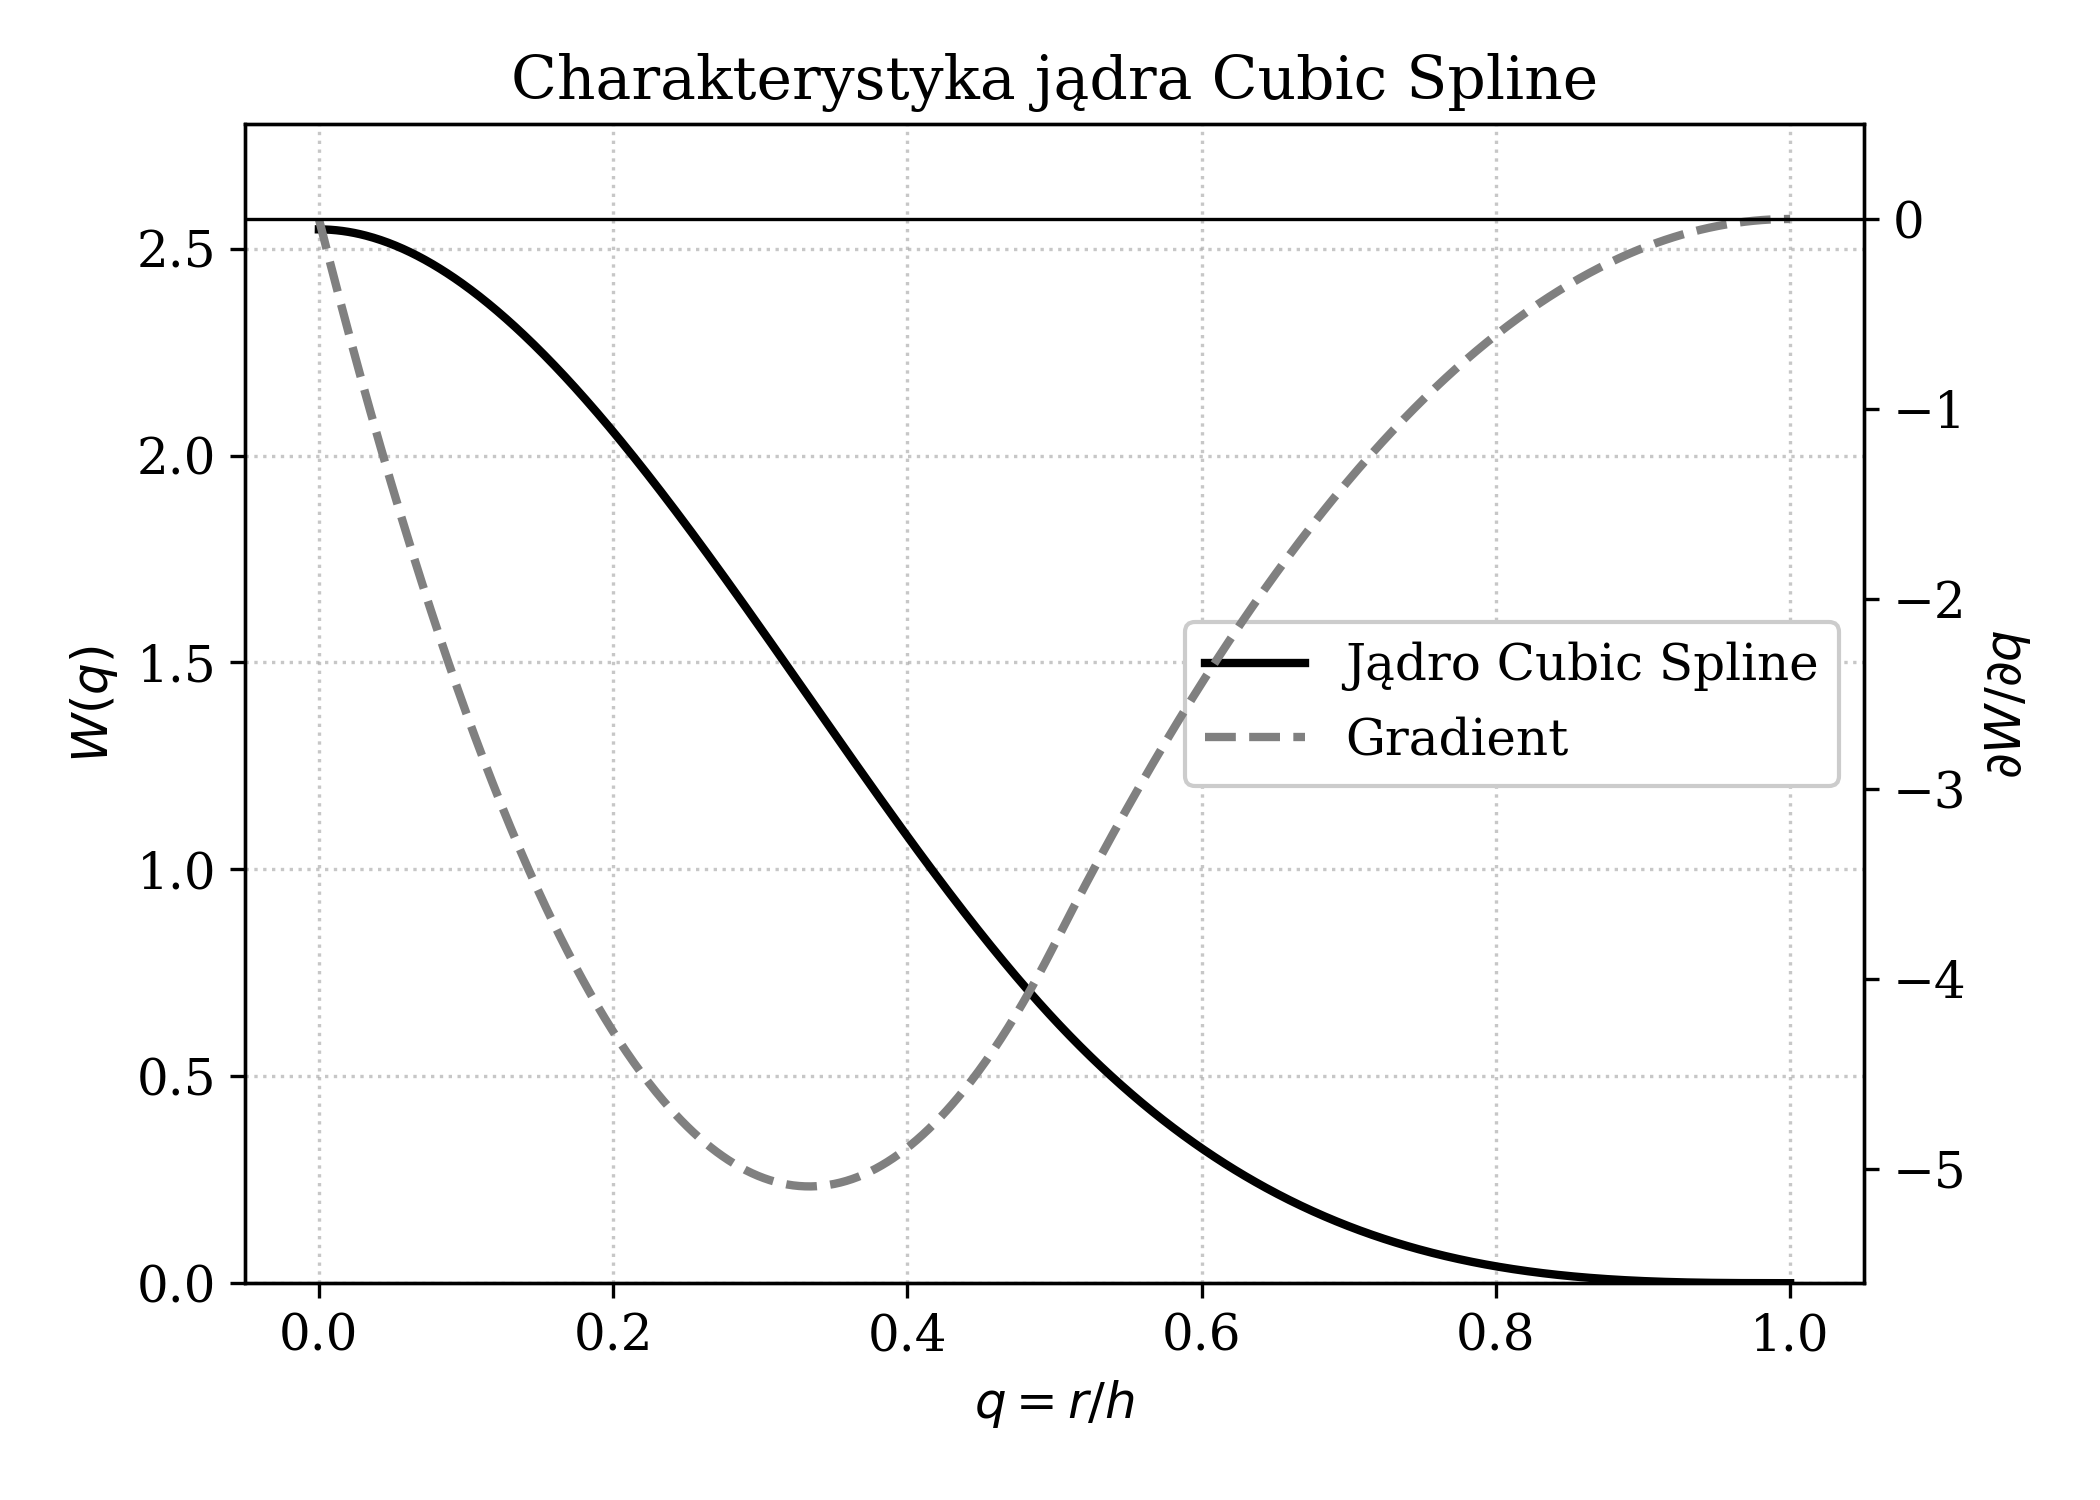
\includegraphics[width=0.72\textwidth]{figures/kernel_cubic_bw.png}
    \caption{Wartość $W(q)$ oraz pochodna radialna $\partial W/\partial q$ sześciennej
    funkcji sklejanej w~funkcji znormalizowanej odległości $q = r/h$
    \newline Źródło: Opracowanie własne na podstawie \cite{koschier2020smoothed}}
    \label{fig:kernel_cubic}
\end{figure}

\subsection{Funkcja Wendlanda C2}

Jądro Wendlanda C2 (ang.~\textit{Wendland quintic C2 kernel}) pochodzi z teorii
radialnych funkcji bazowych \cite{wendland1995piecewise}. W trójwymiarowej przestrzeni
przyjmuje postać wielomianu piątego stopnia:

\begin{equation}
    W(q,\,h) = \frac{21}{2\pi h^3}
    \begin{cases}
        (1-q)^4(4q+1) & \text{dla } 0 \leq q \leq 1, \\
        0              & \text{dla } q > 1,
    \end{cases}
    \label{eq:wendland_kernel}
\end{equation}

a jego gradient przestrzenny:

\begin{equation}
    \nabla W(\mathbf{r},\,h) = -\frac{210}{\pi h^3}
    \begin{cases}
        q(1-q)^3\,\dfrac{\mathbf{r}}{r\,h} & \text{dla } 0 < q \leq 1, \\[6pt]
        \mathbf{0}                           & \text{dla } q > 1.
    \end{cases}
    \label{eq:wendland_grad}
\end{equation}

W odróżnieniu od jądra sześciennego, funkcja Wendlanda C2 jest jednym wyrażeniem
wielomianowym na całym nośniku, bez wewnętrznych punktów sklejenia.
Posiada gwarantowaną dodatniość i monotonicznie malejący profil, a gradient zaczyna się
od zera w $q = 0$, osiąga maksimum w pewnym $q \in (0,\,1)$ i powraca do zera na granicy
nośnika, co ilustruje rysunek~\ref{fig:kernel_wendland}.

\begin{figure}[ht]
    \centering
    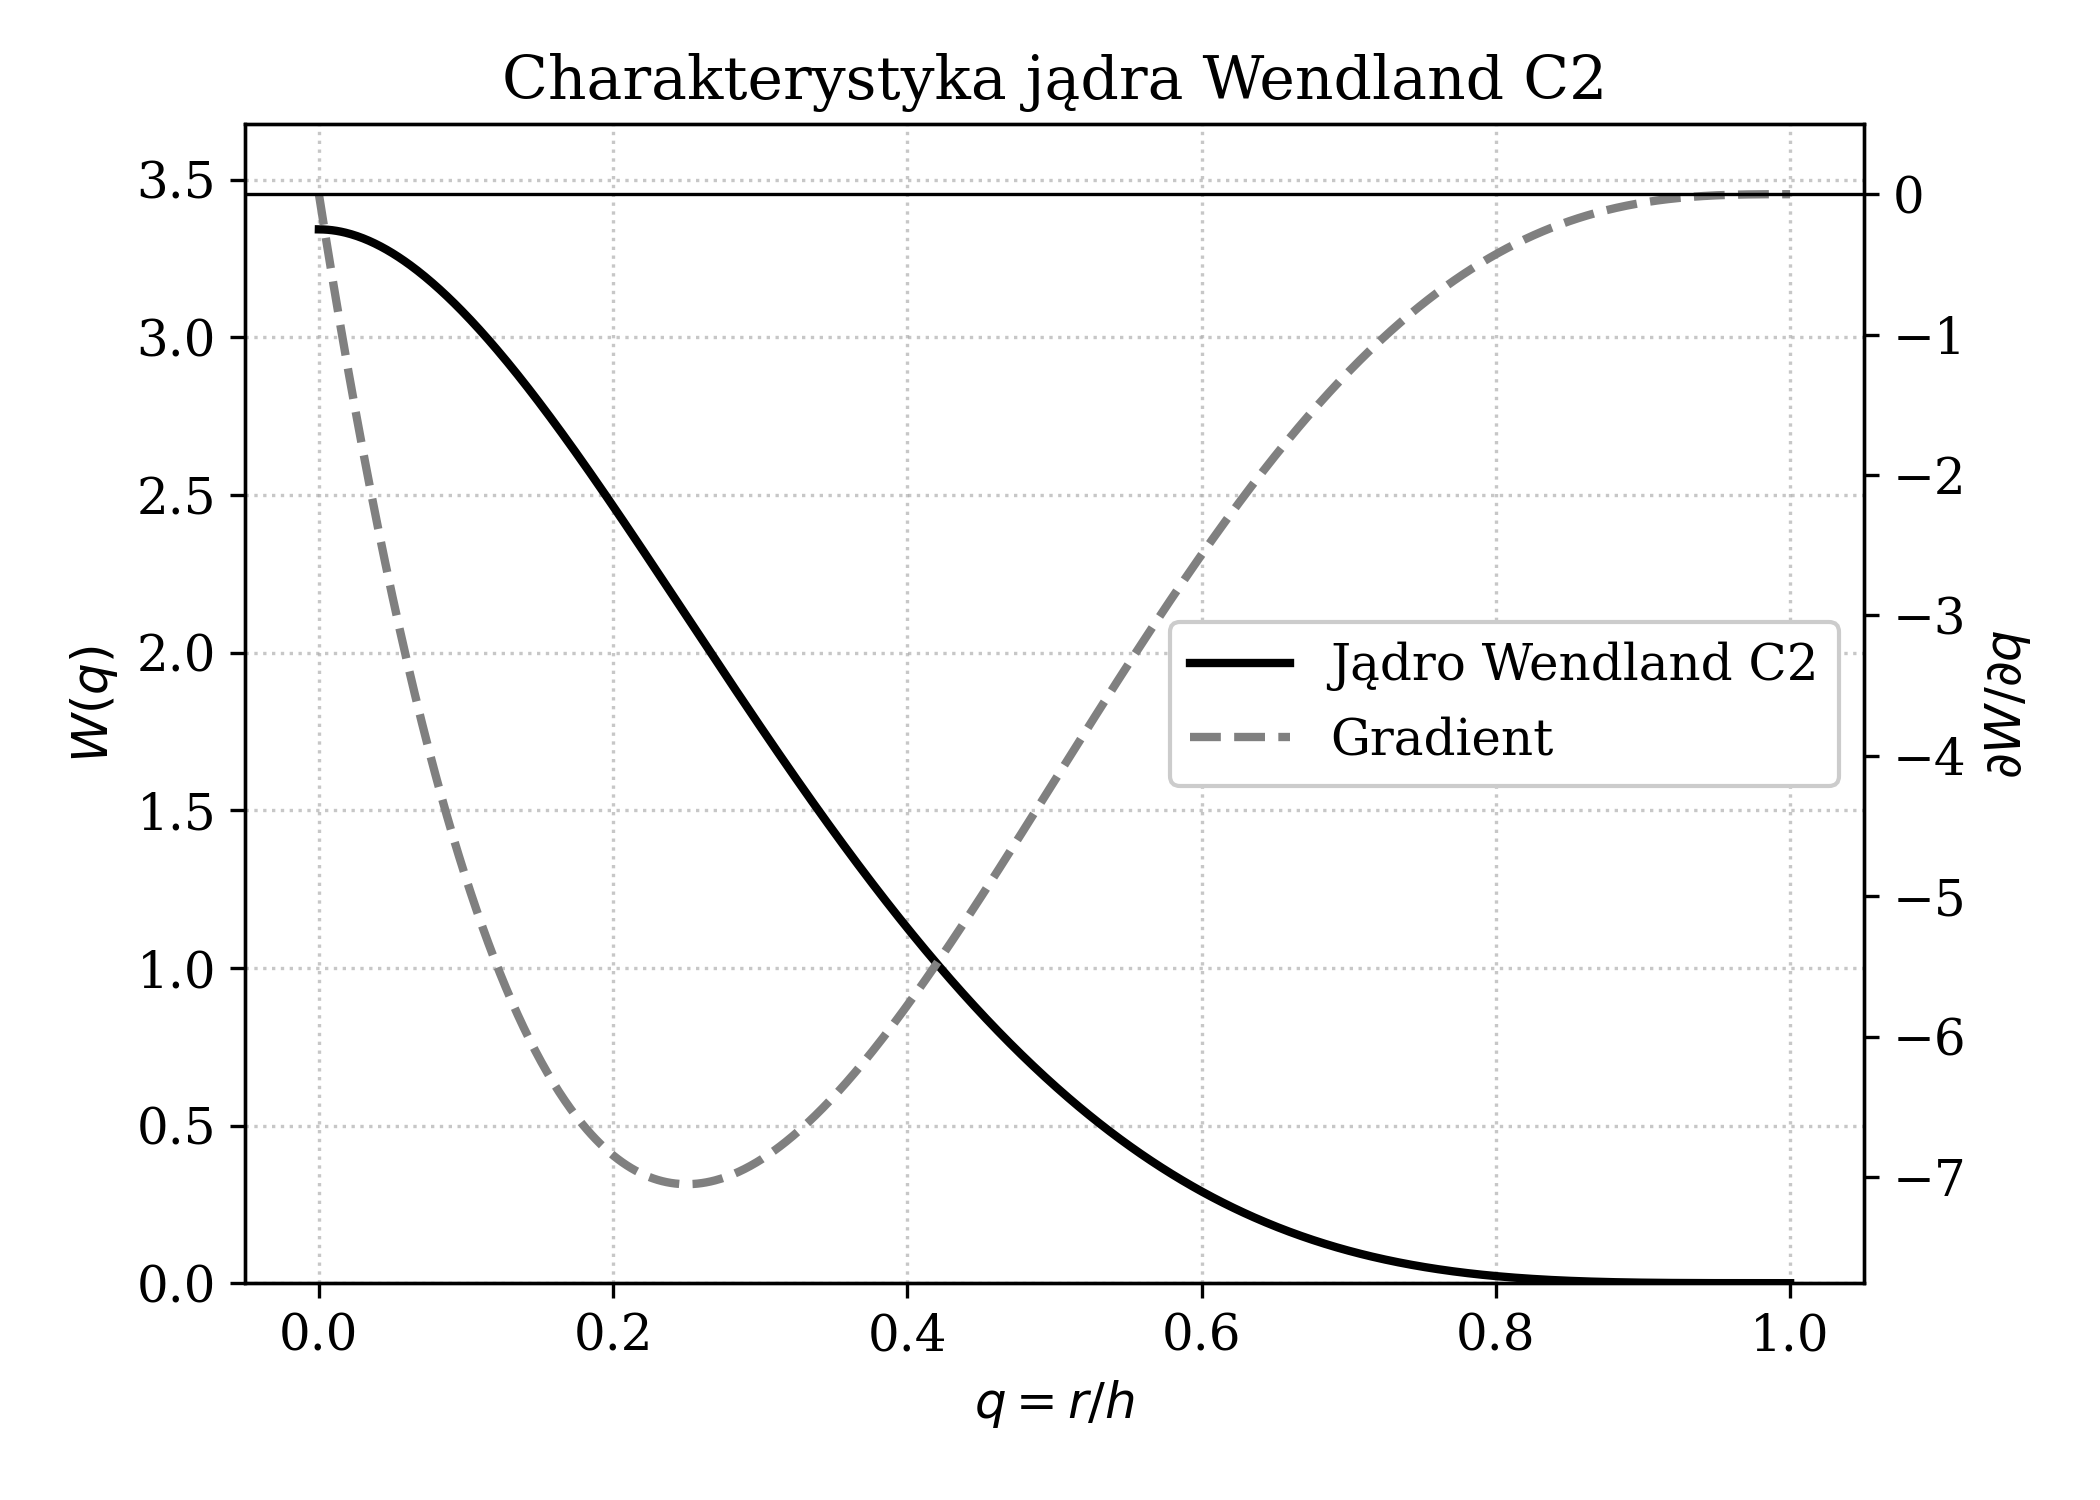
\includegraphics[width=0.72\textwidth]{figures/kernel_wendland_bw.png}
    \caption{Wartość $W(q)$ oraz pochodna radialna $\partial W/\partial q$ jądra
    Wendlanda C2 w funkcji znormalizowanej odległości $q = r/h$
    \newline Źródło: Opracowanie własne na podstawie \cite{wendland1995piecewise}}
    \label{fig:kernel_wendland}
\end{figure}

\subsection{Dobór jądra dla solvera DFSPH}

Porównując oba jądra pod kątem ich zachowania w pobliżu zera, widoczna jest zasadnicza
różnica wynikająca bezpośrednio z rysunków~\ref{fig:kernel_cubic}
i~\ref{fig:kernel_wendland}. Gradient sześciennej funkcji sklejanej jest zerowy
w punkcie $q = 0$, co oznacza, że gdy dwie cząsteczki znajdą się bardzo blisko siebie,
siła odpychająca wynikająca z jądra zanika. Prowadzi to do efektu skupiania się cząsteczek
(ang.~\textit{particle clumping}): cząsteczki, które raz do siebie nadmiernie się zbliżą,
nie napotykają wystarczającego oporu obliczeniowego i zaczynają się zagęszczać w sposób
niekontrolowany. Jądro Wendlanda C2 pozbawione jest tej wady: jego gradient rośnie
niemal liniowo od zera przy $q = 0$ i nie posiada płaskiej strefy przy początku
układu współrzędnych, co zapewnia niezerową siłę odpychającą nawet przy bardzo
małych odległościach.

Wydawałoby się to wystarczającym argumentem na korzyść jądra Wendlanda C2, jednak
badanie Lavrova i współpracowników \cite{lavrov2015density} wskazuje na istotny koszt tej
stabilności. Spośród dziesięciu analizowanych jąder SPH w przestrzeni trójwymiarowej,
jądra Wendlanda należą do grupy wymagającej największej liczby cząsteczek sąsiadujących,
aby zapewnić tę samą dokładność reprezentacji gęstości. Różnica w wymaganej liczbie
sąsiadów między jądrami sześciennymi a jądrami Wendlanda wynosi w 3D nawet trzykrotność,
przy czym kontrast ten pogłębia się wraz ze wzrostem liczby wymiarów. W implementacji
GPU, gdzie każda operacja sąsiedztwa przekłada się bezpośrednio na liczbę instrukcji
wykonywanych przez wątek obliczeniowy, szerszy nośnik efektywny jądra Wendlanda oznacza
proporcjonalnie większy koszt obliczeniowy każdego kroku symulacji.

Kluczowym argumentem przesądzającym o wyborze sześciennej funkcji sklejanej jest
właściwość algorytmu DFSPH. Solver rozbieżności, stanowiący rdzeń metody, wymusza
w każdym kroku czasowym warunek zerowej rozbieżności pola prędkości, co zapobiega
akumulacji błędów gęstości już u ich źródła. Cząsteczki nie mają możliwości nabycia
prędkości zbliżającej je do siebie na tyle, by efekt skupiania się stał się problemem,
gdyż solver koryguje prędkości zanim dojdzie do znacznego zaburzenia gęstości.
Główna słabość sześciennej funkcji sklejanej jest zatem neutralizowana przez sam
algorytm. Na zbieżność tego wniosku z praktyką wskazuje fakt, że autorzy algorytmu
DFSPH w oryginalnej publikacji \cite{bender2015divergence} sami posługują się sześcienną
funkcją sklejaną jako jądrem obliczeniowym. Warto przy tym podkreślić dodatkowe
ograniczenie wskazane przez tych samych autorów: oba solvery składające się na metodę
DFSPH, solver gęstości oraz solver rozbieżności, muszą korzystać z tej samej funkcji
wygładzającej \cite{bender2015divergence}. Oznacza to, że wybór jądra nie jest decyzją
lokalną dotyczącą jednego etapu algorytmu, lecz ma podwójny wpływ na koszt obliczeniowy
całego kroku czasowego. Wybór jądra wymagającego szerszego sąsiedztwa, jak Wendland C2,
obciążałby proporcjonalnie oba solvery jednocześnie. Wobec powyższego, w niniejszej
implementacji przyjęto sześcienną funkcję sklejaną jako jądro wygładzające, czerpiąc
korzyść z mniejszej liczby sąsiadów i tym samym niższego kosztu obliczeniowego przy
zachowaniu pełnej stabilności numerycznej gwarantowanej przez solver DFSPH.

% ----------------------------------------------------------------

\section{Wyszukiwanie sąsiedztwa cząsteczek}
\label{sec:neighbor_search_theory}

Każda cząsteczka w metodzie SPH oddziałuje wyłącznie z cząsteczkami znajdującymi się
w odległości nie większej niż promień wygładzania $h$. Poza tym promieniem wartość
jądra jest równa zero i dana para cząsteczek nie wnosi żadnego wkładu do sum
interpolacyjnych. Wyznaczenie zbioru sąsiadów jest zatem fundamentalnym krokiem
obliczeniowym wykonywanym co najmniej raz na krok czasowy, a przy iteracyjnych
solverach nieściśliwości, takich jak DFSPH, listy sąsiedztwa są wielokrotnie
odczytywane w każdej klatce.

Naiwne podejście, polegające na sprawdzeniu każdej pary cząsteczek, ma złożoność
$\mathcal{O}(N^2)$, gdzie $N$ jest liczbą cząsteczek. Dla symulacji zawierającej
$10^5$ cząsteczek oznacza to $10^{10}$ porównań na krok, co jest w praktyce
nieakceptowalne. Rozwiązaniem jest zastosowanie przestrzennej struktury danych,
które ograniczają proces wyszukiwania do najbliższego otoczenia cząsteczki, 
redukując złożoność zapytania do $\mathcal{O}(1)$ lub $\mathcal{O}(\log N)$.
Najszerzej stosowaną klasą takich struktur w metodzie SPH są siatki jednolite
(ang.~\textit{uniform grids}), których rozmiar komórki dobierany jest równy
promieniowi wygładzania $h$. Wówczas sąsiedzi danej cząsteczki mogą znajdować
się wyłącznie w~sąsiednich komórkach siatki, co w przestrzeni trójwymiarowej
ogranicza przeszukiwany obszar do co najwyżej $27$ komórek niezależnie od $N$.

\subsection{Siatka haszująca według Simona Greena}

Podejście zaproponowane przez Simona Greena \cite{green2010particle} jest
praktyczną realizacją idei siatki jednolitej przystosowaną do masowego
zrównoleglenia na GPU. Przestrzeń symulacji dzielona jest na sześcienne komórki
o boku równym $h$. Każda cząsteczka o~pozycji $\mathbf{r}_i$ przypisywana jest
do komórki o współrzędnych całkowitych:
\begin{equation}
    (k,\,l,\,m) = \left\lfloor \frac{\mathbf{r}_i}{h} \right\rfloor,
\end{equation}
a następnie te trzy współrzędne całkowite odwzorowywane są na jeden indeks tablicy
przez funkcję haszującą, co pozwala uniknąć jawnego przechowywania całej siatki
w~pamięci. Tablica haszująca przechowuje dla każdej komórki zakres indeksów
cząsteczek posortowanej tablicy cząsteczek. Budowa struktury sprowadza się do
posortowania cząsteczek według ich indeksu komórki, co na GPU realizowane jest
przez szybkie sortowanie radixowe \cite{green2010particle}.

Wyszukiwanie sąsiadów dla cząsteczki $i$ przebiega przez iterację po wszystkich
$27$ komórkach sąsiednich w trójwymiarowej siatce, pobranie odpowiednich zakresów
z tablicy haszującej i sprawdzenie warunku $\|\mathbf{r}_i - \mathbf{r}_j\| < h$
dla każdego kandydata. Schemat tej procedury ilustruje rysunek~\ref{fig:hashgrid}.

\begin{figure}[ht]
\centering
\begin{tikzpicture}[
  cell/.style={draw=black!40, thin, fill=white, minimum size=1.1cm},
  hcell/.style={draw=black!70, thin, fill=gray!18, minimum size=1.1cm},
  qcell/.style={draw=black!80, thick, fill=gray!35, minimum size=1.1cm},
  particle/.style={circle, fill=black, inner sep=0pt, minimum size=5pt},
  qparticle/.style={circle, fill=black, inner sep=0pt, minimum size=6pt},
  arr/.style={->, >=Stealth, semithick}
]
  \def\s{1.1}

  % Grid 5x5
  \foreach \c in {0,...,4} {
    \foreach \r in {0,...,4} {
      \node[cell] at (\c*\s, \r*\s) {};
    }
  }

  % Highlight 3x3 search region (cols 1-3, rows 1-3)
  \foreach \c in {1,2,3} {
    \foreach \r in {1,2,3} {
      \node[hcell] at (\c*\s, \r*\s) {};
    }
  }

  % Query cell (center)
  \node[qcell] at (2*\s, 2*\s) {};

  % Particles
  \node[particle] at (0.3, 0.2) {};
  \node[particle] at (0.7, 0.85) {};
  \node[particle] at (1.2, 0.3) {};
  \node[particle] at (1.55, 1.0) {};
  \node[particle] at (1.1, 1.5) {};
  \node[particle] at (1.75, 1.7) {};
  \node[particle] at (3.1, 1.35) {};
  \node[particle] at (2.9, 1.85) {};
  \node[particle] at (3.3, 2.5) {};
  \node[particle] at (1.3, 3.1) {};
  \node[particle] at (2.4, 3.3) {};
  \node[particle] at (3.5, 3.5) {};
  \node[particle] at (0.4, 3.8) {};
  \node[particle] at (4.2, 0.5) {};
  \node[particle] at (4.5, 2.8) {};

  % Query particle
  \node[qparticle] (qp) at (2*\s, 2*\s) {};
  \draw[black!60, dashed, thin] (qp) circle (0.95cm);

  % Labels
  \draw[arr, black!50] (2*\s, -0.18) -- (2*\s, 1.85);

  % Brace / annotation for 3x3 region
  \draw[decorate, decoration={brace, amplitude=5pt, mirror}, thick]
    (0.55, -0.6) -- (3.85, -0.6)
    node[midway, below=6pt, font=\scriptsize\sffamily] {27 komórek w 3D};
\end{tikzpicture}
\caption{Schemat wyszukiwania sąsiedztwa metodą siatki haszującej w 2D. Szare komórki
stanowią obszar przeszukiwania (w 3D odpowiada mu $3\times3\times3 = 27$ komórek).
Przerywane kółko oznacza promień wygładzania $h$; cząsteczka zapytania zaznaczona
jest w~komórce centralnej. Jedynie cząsteczki z wyróżnionych komórek są sprawdzane
pod kątem warunku $\|\mathbf{r}_i - \mathbf{r}_j\| < h$
\newline Źródło: Opracowanie własne na podstawie \cite{green2010particle}}
\label{fig:hashgrid}
\end{figure}

Metoda zapewnia złożoność budowy $\mathcal{O}(N)$ i złożoność zapytania
$\mathcal{O}(1)$ niezależną od liczby cząsteczek. Zakłada ona jednak z góry
określony rozmiar tablicy haszującej i stałą domenę symulacji, co jest
akceptowalne dla zamkniętych scen symulacyjnych.

\subsection{Skompresowane listy sąsiedztwa jako alternatywa}

Metodą stanowiącą bardziej nowoczesną alternatywę jest podejście zaproponowane
przez Banda, Gisslera i Teschnera \cite{band2019compressed}, będące wariantem
struktury połączonych list komórek (ang.~\textit{Cell-Linked-List}, CLL).
W odróżnieniu od podejścia Greena, siatka nie jest jawnie reprezentowana w
pamięci: przechowywana jest jedynie zwarta lista niepustych komórek, co eliminuje
koszt pamięciowy rzadko wypełnionych domen i umożliwia obsługę nieograniczonych
dziedzin przestrzennych bez z góry zdefiniowanego rozmiaru siatki.

Kluczowym elementem metody jest posortowanie cząsteczek według indeksu komórki
wyznaczonego krzywą Mortona, przestrzenną krzywą wypełniającą odwzorowującą
współrzędne komórki na jednowymiarowy indeks tak, by sąsiednie przestrzennie
cząsteczki trafiały do sąsiednich pozycji w tablicy. Poprawia to lokalność danych
w~pamięci podręcznej podczas iteracji po listach sąsiedztwa, co ilustruje
rysunek~\ref{fig:cll}.

\begin{figure}[ht]
\centering
\begin{tikzpicture}[
  pbox/.style={draw=black!70, fill=white, minimum width=0.72cm,
               minimum height=0.62cm, align=center, font=\scriptsize\ttfamily},
  cbox/.style={draw=black!70, fill=gray!14, minimum width=0.72cm,
               minimum height=0.62cm, align=center, font=\scriptsize\ttfamily},
  hbox/.style={draw=black!80, fill=gray!30, minimum width=0.72cm,
               minimum height=0.62cm, align=center, font=\scriptsize\ttfamily},
  arr/.style={->, >=Stealth, semithick},
  lbl/.style={font=\scriptsize\sffamily}
]
  % Sorted particle array
  \node[lbl, anchor=east] at (-0.4, 1.5) {cząsteczki};
  \foreach[count=\i from 0] \c in {2,2,3,3,3,5,5,7,7,7,7,9} {
    \pgfmathsetmacro{\ishigh}{(\c==3||(\c==7)) ? 1 : 0}
    \ifnum\c=3
      \node[hbox] at (\i*0.74, 1.5) {\i};
    \else
      \ifnum\c=7
        \node[hbox] at (\i*0.74, 1.5) {\i};
      \else
        \node[pbox] at (\i*0.74, 1.5) {\i};
      \fi
    \fi
  }

  % Cell indices below
  \node[lbl, anchor=east] at (-0.4, 0.75) {komórka};
  \foreach[count=\i from 0] \c in {2,2,3,3,3,5,5,7,7,7,7,9} {
    \ifnum\c=3
      \node[hbox] at (\i*0.74, 0.75) {\c};
    \else
      \ifnum\c=7
        \node[hbox] at (\i*0.74, 0.75) {\c};
      \else
        \node[cbox] at (\i*0.74, 0.75) {\c};
      \fi
    \fi
  }

  % Compact cell array
  \node[lbl, anchor=east] at (-0.6, -0.1) {zwarta lista komórek};
  \foreach[count=\i from 0] \entry in {{2:0},{3:2},{5:5},{7:7},{9:11}} {
    \node[cbox, minimum width=1.3cm] at (\i*1.36, -0.1) {\entry};
  }

  \node[lbl, anchor=west] at (6.95, 1.5) {\dots};
  \node[lbl, anchor=west] at (6.95, 0.75) {\dots};

  \node[lbl, font=\scriptsize\itshape] at (3.4, -0.65)
    {format: indeks\_komórki : pierwszy\_indeks\_cząsteczki};
\end{tikzpicture}
\caption{Schemat struktury CLL z kompaktową tablicą komórek. Górny wiersz zawiera
indeksy cząsteczek posortowane według indeksu komórki (wyznaczonego krzywą Mortona);
środkowy wiersz pokazuje odpowiadające indeksy komórek; dolny wiersz przedstawia
zwartą tablicę komórek przechowującą wyłącznie niepuste komórki z odniesieniem do
pierwszej cząsteczki w posortowanej tablicy. Wyróżnione (szare) pola odpowiadają
przykładowym komórkom 3 i 7
\newline Źródło: Opracowanie własne na podstawie \cite{band2019compressed}}
\label{fig:cll}
\end{figure}

Drugą cechą wyróżniającą metodę jest kompresja list sąsiedztwa. Ponieważ
cząsteczki są posortowane, indeksy sąsiadów są niemalejące, a ich różnice
są małe. Autorzy wykorzystują tę właściwość, kodując różnice kolejnych
indeksów sąsiadów za pomocą schematu inspirowanego algorytmem StreamVByte,
osiągając oszczędność pamięci sięgającą $87\%$ w porównaniu z nieskompresowaną
reprezentacją. W iteracyjnych solverach nieściśliwości, takich jak DFSPH,
gdzie listy sąsiedztwa są wielokrotnie odczytywane w każdym kroku, przechowywanie
skompresowanych list i ich odczytywanie na żądanie jest naturalnym rozwiązaniem.
Metoda ta jest szczególnie korzystna dla dużych symulacji w otwartych scenach,
gdzie domena nie jest z góry ograniczona, a siatka haszująca wymagałaby rozbudowanej
tablicy. Jej implementacja opisana w \cite{band2019compressed} jest ukierunkowana
na procesory wielordzeniowe; autorzy wskazują implementację GPU jako kierunek
dalszych badań. Z tego względu, przy implementacji opartej w całości na GPU,
zastosowano prostsze podejście siatki haszującej opisane w podrozdziale poprzednim.

% ----------------------------------------------------------------

\section{Modelowanie zjawisk fizycznych}
\label{sec:physical_models_theory}

Równanie pędu Naviera-Stokesa zawiera trzy człony siłowe: gradient ciśnienia,
naprężenia lepkie oraz siły zewnętrzne. Solver DFSPH, opisany w poprzednich
rozdziałach, rozwiązuje wyłącznie człon ciśnieniowy, wymuszając nieściśliwość.
Pozostałe zjawiska fizyczne, mianowicie opór lepki, kohezja cząsteczek na
powierzchni swobodnej oraz oddziaływanie z granicami domeny, wymagają osobnych
modeli dyskretnych. Każde z nich może być pominięte w minimalnej implementacji
solvera, lecz każde odpowiada za inny aspekt fizycznej poprawności symulacji.
W niniejszej sekcji omówiono teoretyczne podstawy tych modeli.

\subsection{Lepkość}

Lepkość jest miarą wewnętrznego oporu cieczy na odkształcenie ścinające. W równaniu
pędu odpowiada za nią tensor naprężeń dewiacyjnych $\boldsymbol{\tau}$. Dla cieczy
newtonowskich tensor ten jest proporcjonalny do symetrycznego gradientu prędkości:
\begin{equation}
    \boldsymbol{\tau} = \mu \left( \nabla \mathbf{u} + (\nabla \mathbf{u})^\top \right),
\end{equation}
gdzie $\mu$ jest dynamicznym współczynnikiem lepkości. Dywergencja tego tensora
wchodzi do równania pędu jako przyspieszenie lepkie $\mathbf{a}^{\mathrm{visc}}$.
W dyskretyzacji SPH najczęściej stosowanym podejściem jest sformułowanie Morrisa
i współpracowników \cite{morris1997modeling}, które zastępuje człon
$\nabla \cdot \boldsymbol{\tau}$ operatorem opartym na laplasjanie prędkości:
\begin{equation}
    \mathbf{a}^{\mathrm{visc}}_i = \frac{\mu}{\rho_i}
    \sum_j \frac{m_j}{\rho_j} \, (\mathbf{v}_j - \mathbf{v}_i)
    \frac{1}{r_{ij}} \frac{\partial W_{ij}}{\partial r},
\end{equation}
gdzie $r_{ij} = \|\mathbf{r}_i - \mathbf{r}_j\|$. Wyraz ten tłumi względne
prędkości sąsiadów proporcjonalnie do odległości, modelując dyssypację energii
kinetycznej charakterystyczną dla cieczy lepkich. Brak członu lepkiego sprawia,
że ciecz zachowuje się jak idealna, zachowując energię mechaniczną bez strat,
co jest fizycznie nierealistyczne dla większości cieczy, choć nie destabilizuje
solvera.

Odrębnym mechanizmem pokrewnym lepkości jest korekcja XSPH \cite{monaghan1989problem},
w której prędkość cząsteczki jest nieznacznie uśredniana względem prędkości jej
sąsiadów. Nie modeluje ona jawnie dyssypacji energii, lecz wygładza pole prędkości,
zapobiegając przenikaniu i lokalnym skupieniom cząsteczek. Mechanizm ten działa
niezależnie od fizycznej lepkości i może być stosowany zarówno przy $\mu = 0$,
jak i przy niezerowej jej wartości.

\subsection{Napięcie powierzchniowe}

Napięcie powierzchniowe jest efektem makroskopowym niezrównoważonych sił kohezji
działających na cząsteczki cieczy leżące przy granicy fazy swobodnej. Cząsteczka
w głębi cieczy jest otoczona sąsiadami ze wszystkich stron i suma sił kohezji
znosi się; cząsteczka na powierzchni ma sąsiadów tylko po stronie cieczy, co
wytwarza wypadkową siłę skierowaną do jej wnętrza. Efektem jest minimalizacja
pola powierzchni swobodnej i charakterystyczny kształt kropli.

W sformułowaniu opartym na równaniu Younga-Laplace'a \cite{batchelor1967introduction}
różnica ciśnienia po obu stronach zakrzywionej powierzchni wynosi:
\begin{equation}
    \Delta p = \gamma \kappa,
\end{equation}
gdzie $\gamma$ jest współczynnikiem napięcia powierzchniowego, a $\kappa$ krzywizną
powierzchni. W metodzie SPH krzywizna wyznaczana jest na podstawie pola normalnego
szacowanego z gradientu jądra, a wypadkowa siła kohezji przykładana jest jako
przyspieszenie cząsteczek leżących przy powierzchni. Bez napięcia powierzchniowego
symulacja pozostaje stabilna, lecz traci zdolność do formowania kropli i
realistycznego zachowania cienkiej warstwy cieczy. W niniejszej pracy napięcie
powierzchniowe nie zostało zaimplementowane; symulowane sceny obejmują swobodną
powierzchnię bez zjawisk kapilarnych, gdzie jego pominięcie nie wpływa istotnie
na poprawność wyników \cite{koschier2020smoothed}.

\subsection{Warunki brzegowe}

Granice domeny symulacji wprowadzają fundamentalny problem geometryczny: cząsteczka
znajdująca się w pobliżu ściany ma niepełny obszar wsparcia jądra, ponieważ część
sfery sąsiedztwa o promieniu $h$ wychodzi poza domenę i nie zawiera żadnych
cząsteczek. Sytuację tę ilustruje rysunek~\ref{fig:boundary_support}.

\begin{figure}[ht]
\centering
\begin{tikzpicture}[scale=1.3,
  particle/.style={circle, fill=black, inner sep=0pt, minimum size=5pt},
  ghost/.style={circle, draw=black!40, fill=gray!15, inner sep=0pt,
                minimum size=5pt, dashed},
  arr/.style={->, >=Stealth, semithick}
]
  % Wall (hatch fill)
  \fill[gray!20] (-0.5, -0.5) rectangle (0.5, 2.5);
  \draw[thick] (0.5, -0.5) -- (0.5, 2.5);
  \foreach \y in {-0.3, 0.1, 0.5, 0.9, 1.3, 1.7, 2.1} {
    \draw[black!30, thin] (0.1, \y) -- (0.5, \y+0.4);
  }
  \node[font=\scriptsize\sffamily, rotate=90] at (0.0, 1.0) {ściana};

  % Query particle
  \node[particle, fill=black] (qp) at (1.3, 1.0) {};
  \node[font=\scriptsize\sffamily, above=3pt] at (qp) {$i$};

  % Support radius circle
  \draw[black, dashed, thin] (qp) circle (1.2cm);
  \node[font=\scriptsize\sffamily] at (2.6, 1.85) {$h$};

  % Fluid particles (only on fluid side)
  \node[particle] at (1.7, 0.3) {};
  \node[particle] at (2.1, 1.1) {};
  \node[particle] at (1.6, 1.7) {};
  \node[particle] at (2.3, 0.6) {};
  \node[particle] at (1.9, 1.7) {};

  % Missing region annotation
  \draw[black!50, thin, <->] (0.5, -0.3) -- (1.3, -0.3)
    node[midway, below, font=\scriptsize\sffamily] {brak sąsiadów};

  % Ghost particles (mirror)
  \node[ghost] at (0.9, 0.3) {};
  \node[ghost] at (0.5, 1.0) {};
  \node[ghost] at (0.9, 1.7) {};
  \node[font=\scriptsize\sffamily, black!50] at (-0.1, 0.4)
    {\textit{duch}};
\end{tikzpicture}
\caption{Problem niepełnego sąsiedztwa przy granicy domeny. Sfera wsparcia
cząsteczki $i$ przecina ścianę; brak sąsiadów po lewej stronie prowadzi do
zaniżenia oszacowania gęstości i błędu gradientu ciśnienia. Cząsteczki-duchy
(szare, przerywane) uzupełniają brakujący obszar wsparcia
\newline Źródło: Opracowanie własne na podstawie \cite{schechter2012ghost}}
\label{fig:boundary_support}
\end{figure}

Konsekwencje niekompletnego sąsiedztwa są wielorakie. Gęstość wyznaczana sumą
SPH jest zaniżona względem wartości spoczynkowej $\rho_0$, co powoduje, że solver
ciśnienia generuje w pobliżu ścian fałszywy gradient przyciągający cząsteczki do
granicy. Gradient ciśnienia jest dodatkowo błędnie skierowany, ponieważ suma
po sąsiadach nie jest symetrycznie rozkładana wokół cząsteczki. Przy dużych
krokach czasowych możliwe jest też przenikanie cząsteczek przez ścianę.

Powszechnym rozwiązaniem w literaturze są cząsteczki-duchy \cite{schechter2012ghost},
tworzone symetrycznie po drugiej stronie granicy jako odbicia cząsteczek fluidu.
Uzupełniają one brakujący obszar wsparcia, przywracając symetrię sumy SPH, i mogą
być wyposażone w odwróconą prędkość normalną, modelując sprężyste lub lepkie odbicie
od ściany. Alternatywą są stałe warstwy cząsteczek brzegowych reprezentujące
geometrię przeszkody, których cząsteczki uczestniczą w sumach SPH, lecz nie podlegają
integracji ruchu. W niniejszej pracy zastosowano uproszczone podejście: po każdym
kroku całkowania pozycja cząsteczek przekraczających granicę domeny jest korygowana
do jej wnętrza, a składowa normalna prędkości jest odbijana.

% ----------------------------------------------------------------

\section{Potok wizualizacji}
\label{sec:visualization_pipeline_theory}

Wynikiem każdego kroku symulacji DFSPH jest zbiór $N$ cząsteczek z~zaktualizowanymi
pozycjami. Cząsteczki stanowią dyskretne punkty masy; same w sobie nie tworzą
żadnej ciągłej powierzchni, którą mógłby przetworzyć renderer. Aby uzyskać
fotorealistyczny obraz cieczy, potok wizualizacji wykonuje trzy kolejne etapy:
rekonstrukcję ciągłego pola gęstości ze zbioru punktów, wyznaczenie niejawnej
izopowierzchni metodą raymarching oraz obliczenie koloru piksela z~uwzględnieniem
fizycznych właściwości optycznych wody. Ogólną strukturę potoku ilustruje
rysunek~\ref{fig:vis_pipeline}.

\begin{figure}[ht]
\centering
\begin{tikzpicture}[
  box/.style={rectangle, draw=black, thick, rounded corners=3pt,
              minimum width=2.6cm, minimum height=0.85cm,
              font=\small\sffamily, align=center, inner sep=5pt},
  arr/.style={->, >=Stealth, thick}
]
  \node[box] (sim) at (0,    0)   {Cząsteczki\\SPH};
  \node[box] (spl) at (3.6,  0)   {Splatting\\(siatka wokseli)};
  \node[box] (tex) at (7.2,  0)   {3D tekstura\\gęstości};
  \node[box] (ray) at (10.8, 0)   {Raymarching\\(izopowierzchnia)};
  \node[box] (shd) at (10.8,-2.0) {Model\\optyczny};
  \node[box] (px)  at (7.2, -2.0) {Kolor\\piksela};
  \draw[arr] (sim) -- (spl);
  \draw[arr] (spl) -- (tex);
  \draw[arr] (tex) -- (ray);
  \draw[arr] (ray) -- (shd);
  \draw[arr] (shd) -- (px);
\end{tikzpicture}
\caption{Potok wizualizacji: od listy cząsteczek SPH do końcowego koloru piksela
\newline Źródło: Opracowanie własne}
\label{fig:vis_pipeline}
\end{figure}

\subsection{Rekonstrukcja pola gęstości}

Pierwszym krokiem potoku jest przekształcenie listy pozycji cząsteczek w~trójwymiarową
teksturę wolumetryczną \cite{kaufman2005overview}. Domenę symulacji dzieli się na
regularną siatkę wokseli o~rozdzielczości $G_x \times G_y \times G_z$, gdzie każdy
woksel przechowuje skumulowaną gęstość wyrażoną liczbą całkowitą. Dla każdej
cząsteczki $i$ wyznaczany jest odpowiadający jej woksel centralny $\mathbf{c}_i$,
a~następnie do każdego woksela $\mathbf{c}$ w promieniu $R$ wokseli dodawana jest
waga:
\begin{equation}
    w(\delta) = \left(1 - \left(\frac{\delta}{R}\right)^{\!2}\right)^{\!3},
    \qquad \delta = \|\mathbf{c} - \mathbf{c}_i\|.
    \label{eq:splat_weight}
\end{equation}
Funkcja ta jest gładkim wielomianem wygasającym do zera na granicy kuli, co
gwarantuje ciągłość pola bez nieciągłości widocznych jako artefakty wizualne.

Ponieważ każda cząsteczka przetwarzana jest przez osobny wątek GPU, wiele wątków
może jednocześnie aktualizować ten sam woksel. Konflikty zapisu rozwiązuje
instrukcja atomowa \texttt{imageAtomicAdd}, która gwarantuje spójność sumy bez
konieczności synchronizacji. Wynikiem etapu splatting jest trójwymiarowa tekstura
liczb całkowitych: woksele wewnątrz masy cieczy osiągają wartości rzędu setek,
woksele powietrza zbliżone są do zera. Granica między tymi obszarami stanowi
niejawną definicję powierzchni cieczy.

\subsection{Raymarching izopowierzchni}

Mając pole gęstości $\rho(\mathbf{p})$ zapisane w~teksturze 3D, powierzchnię
cieczy definiuje się jako izopowierzchnię:
\begin{equation}
    S = \bigl\{\,\mathbf{p} \in \mathbb{R}^3 : \rho(\mathbf{p}) = \rho_{\mathrm{thr}}\,\bigr\}.
\end{equation}
Wyznaczenie przecięcia promienia kamery z~tą powierzchnią realizuje metoda
raymarching \cite{quilez2008raymarching, tomczak2012gpu}: promień emitowany ze
środka projekcji przemieszcza się równomiernymi krokami $\Delta t$ wzdłuż swojego
kierunku, w każdym punkcie próbkując teksturę, aż wartość gęstości przekroczy próg.
Przed rozpoczęciem marszowania wykonywany jest test przecięcia promienia
z~prostopadłościanem wyrównanym do osi (ang.~\textit{Axis-Aligned Bounding Box}, AABB), czyli
minimalnym prostopadłościanem wyrównanym do osi układu współrzędnych,
który szczelnie otacza domenę symulacji. Test ten, oparty na metodzie płaszczyzn
równoległych, wyznacza w~sposób analityczny zakres
parametru $t \in [t_{\min},\, t_{\max}]$ odpowiadający wejściu i~wyjściu promienia
z~domeny; promienie nie trafiające w~AABB odrzucane są na poziomie shadera
fragmentów, zanim pętla marszowania w~ogóle się rozpocznie.

Próbkowanie tekstury odbywa się z~ręczną interpolacją trójliniową ośmiu sąsiednich
tekseli, zapewniającą ciągłość sygnału niezbędną do poprawnego wyliczenia normalnych.
Aby uniknąć pominięcia cienkiej warstwy cieczy przy dużym kroku, po wykryciu
pierwszego przekroczenia progu wykonuje się ośmiokrotną bisekcję przedziału
$[t_{\mathrm{prev}},\, t_{\mathrm{hit}}]$, lokalizując punkt powierzchni z~dokładnością
$\Delta t\,/\,2^8$ bez zmniejszania globalnego kroku. Schemat algorytmu ilustruje
rysunek~\ref{fig:raymarching}.

\begin{figure}[ht]
\centering
\begin{tikzpicture}[scale=1.05,
  miss/.style={circle, draw=black, fill=white, inner sep=0pt, minimum size=7pt},
  hit/.style={circle, fill=black!55, inner sep=0pt, minimum size=7pt}
]
  % Fluid blob (ellipse, left edge at x = 5.8 - 1.9 = 3.9)
  \fill[gray!15] (5.8, 0) ellipse (1.9cm and 1.1cm);
  \draw[thick]   (5.8, 0) ellipse (1.9cm and 1.1cm);
  \node[font=\scriptsize\sffamily, gray!70] at (5.8, 0) {ciecz};
  \node[font=\scriptsize\sffamily] at (2.0, 1.3) {izopowierzchnia};
  \draw[->, gray!60, thin] (2.65, 1.2) -- (3.65, 0.6);

  % Camera
  \filldraw[black] (-0.2, 0) circle (2.5pt);
  \node[font=\footnotesize\sffamily, below=3pt] at (-0.2,0) {kamera};

  % Ray
  \draw[->, >=Stealth, thick] (-0.2, 0) -- (8.2, 0)
    node[right, font=\scriptsize\sffamily] {promień};

  % Miss samples (x < 3.9)
  \node[miss] at (0.8, 0) {};
  \node[miss] at (1.7, 0) {};
  \node[miss] at (2.6, 0) {};
  \node[miss] at (3.5, 0) {};
  \node[font=\scriptsize\sffamily, above=4pt] at (3.5, 0) {$t_4$};

  % Hit sample (x = 4.4, inside ellipse since 4.4 > 3.9)
  \node[hit] at (4.4, 0) {};
  \node[font=\scriptsize\sffamily, above=4pt] at (4.4, 0) {$t_5$};

  % Binary search bracket
  \draw[<->, >=Stealth, gray, semithick] (3.5,-0.52) -- (4.4,-0.52)
    node[midway, below, font=\scriptsize\sffamily, gray] {bisekcja $\times 8$};

  % True surface point (left edge of ellipse at x=3.9)
  \draw[dashed, black!40] (3.9,-0.72) -- (3.9, 0.65);
  \filldraw[black] (3.9, 0) circle (2.5pt);
  \node[font=\scriptsize\sffamily, above=4pt] at (3.9, 0) {$\mathbf{p}_s$};

  % Normal arrow
  \draw[->, >=Stealth, thick] (3.9, 0) -- (3.0, 0.75)
    node[above left, font=\scriptsize\sffamily] {$\mathbf{N}$};
\end{tikzpicture}
\caption{Schemat raymarchingu z~binarnym zawężaniem. Białe kółka to próbki poniżej
         progu gęstości (powietrze), szare kółko to pierwsza próbka powyżej progu
         (ciecz). Bisekcja przedziału $[t_4,\, t_5]$ wyznacza punkt powierzchni
         $\mathbf{p}_s$ z~dokładnością $\Delta t / 2^8$
         \newline Źródło: Opracowanie własne na podstawie \cite{quilez2013advancing}}
\label{fig:raymarching}
\end{figure}

Normalna powierzchni wyznaczana jest metodą różnic skończonych na polu gęstości~\cite{tomczak2012gpu}:
\begin{equation}
    \mathbf{N}(\mathbf{p}) = -\,\nabla\rho(\mathbf{p}) \approx -\frac{1}{2\varepsilon}
    \begin{pmatrix}
        \rho(\mathbf{p}+\varepsilon\hat{x}) - \rho(\mathbf{p}-\varepsilon\hat{x}) \\[2pt]
        \rho(\mathbf{p}+\varepsilon\hat{y}) - \rho(\mathbf{p}-\varepsilon\hat{y}) \\[2pt]
        \rho(\mathbf{p}+\varepsilon\hat{z}) - \rho(\mathbf{p}-\varepsilon\hat{z})
    \end{pmatrix}.
\end{equation}
Podejście to nie wymaga jawnej siatki trójkątów i~automatycznie odzwierciedla
bieżącą topologię pola gęstości, co jest kluczowe przy dynamicznie zmieniającej
się powierzchni cieczy.

\subsection{Model optyczny cieczy}

Woda jest dielektrycznym, częściowo transparentnym ośrodkiem, w~którym na powierzchni
jednocześnie zachodzi odbicie i~załamanie światła, a~wewnątrz objętości promienie
ulegają absorpcji i~rozproszeniu \cite{pharr2016physically}. Poniżej omówiono kolejno
efekty zaimplementowane w~shaderze fragmentów.

\textbf{Środowisko HDRI.} Otoczenie sceny reprezentuje sferyczna mapa środowiskowa
w~formacie równokątnym (ang.~\textit{equirectangular}), próbkowana przez osobny shader
nieba. Każde odbicie i~załamanie na powierzchni wody próbkuje tę samą teksturę
w~przeliczonym kierunku, zapewniając spójność oświetlenia między cieczą a~tłem.

\textbf{Efekt Fresnela.} Stosunek energii odbitej do załamanej zależy od kąta
padania i~właściwości dielektrycznych ośrodka \cite{de2006reflections}. Dla wody
o~współczynniku załamania $n = 1{,}333$ odbicie przy normalnym kącie padania wynosi:
\begin{equation}
    F_0 = \left(\frac{n_1 - n_2}{n_1 + n_2}\right)^{\!2} \approx 0{,}02
\end{equation}
i~wzrasta do jedności przy kącie ślizgowym. W~shaderze stosuje się przybliżenie
Schlicka:
\begin{equation}
    F(\theta) = F_0 + (1 - F_0)(1 - \cos\theta)^5,
\end{equation}
gdzie $\theta$ jest kątem między wektorem widoku $\mathbf{V}$ a~normalną $\mathbf{N}$.
Kierunek odbitego promienia próbkuje skybox, kierunek załamanego wyznaczany jest
prawem Snella. Końcowy kolor piksela to interpolacja liniowa między kolorem
załamania a~odbicia z~wagą $F$.

\textbf{Absorpcja Beer-Lamberta.} Światło przenikające przez grubość cieczy $d$
ulega wykładniczej absorpcji:
\begin{equation}
    \mathbf{c}_{\mathrm{abs}} = \mathbf{c}_{\mathrm{bg}} \cdot
    \exp(-\boldsymbol{\mu}_a \cdot d),
\end{equation}
gdzie $\boldsymbol{\mu}_a = (\mu_R,\, \mu_G,\, \mu_B)$ są kanałowymi współczynnikami
absorpcji. Silna absorpcja czerwonego ($\mu_R = 0{,}45$) przy słabej niebieskiego
($\mu_B = 0{,}025$) nadaje wodzie charakterystyczną niebieskozieloną barwę.
Grubość $d$ wyznaczana jest osobnym przebiegiem promienia od punktu powierzchni
do tylnej ściany AABB.

\textbf{Rozproszenie podpowierzchniowe.} Część energii słonecznej nie jest
pochłaniana, lecz wielokrotnie rozpraszana wewnątrz cieczy i~wychodzi jako miękka
turkusowa poświata widoczna zwłaszcza w~cienkich partiach fali. Efekt modeluje się
przybliżeniem łączącym zawiniętą dyfuzję (ang.~\textit{wrapped diffuse}) z~tylnym
rozproszeniem:
\begin{equation}
    L_{\mathrm{sss}} = c_s \cdot L_{\odot} \cdot
    \bigl(0{,}6\;\sigma_{\mathrm{wrap}} + 0{,}4\;\sigma_{\mathrm{back}}\bigr)
    \cdot \bigl(1 - e^{-3d}\bigr),
\end{equation}
gdzie $\sigma_{\mathrm{wrap}} = \max\bigl(0,\,\mathbf{N}{\cdot}\mathbf{L}\cdot0{,}5+0{,}5\bigr)$
modeluje oświetlenie przechodzące przez krawędź fali, a~$\sigma_{\mathrm{back}} =
\max(0,\,-\mathbf{N}{\cdot}\mathbf{L})$ odpowiada za tylne rozproszenie w~kierunku
obserwatora.

\textbf{Odbłysk spekularny GGX.} Mikrostruktury falującej powierzchni modeluje
rozkład normalnych GGX \cite{walter2007microfacet} o~parametrze szerokości $\alpha = 0{,}04$:
\begin{equation}
    D_{\mathrm{GGX}}(\mathbf{H}, \alpha) =
    \frac{\alpha^2}{\pi\,\bigl[(\mathbf{N}{\cdot}\mathbf{H})^2(\alpha^2-1)+1\bigr]^2},
\end{equation}
gdzie $\mathbf{H} = \mathrm{normalize}(\mathbf{L} + \mathbf{V})$ jest półwektorem
między kierunkiem światła a~wektorem widoku, a~$\alpha$~--- parametrem szerokości
rozkładu GGX odpowiadającym chropowatości powierzchni.

\textbf{Piana i~mapowanie tonalne.} Regiony, w~których normalna jest prawie pionowa
($N_y \approx 1$) przy małej grubości cieczy, maskowane są kolorem pianki,
naśladując bąble powietrza na grzbietach fali. Na koniec kolor HDR przekształcany
jest operatorem Reinharda \cite{reinhard2002photographic}
$\mathbf{c}' = \mathbf{c}\,/\,(1+\mathbf{c})$ do zakresu $[0,1]$ przed zapisem
do bufora ramki.
